\documentclass[10pt,twocolumn]{article}
\usepackage{cite}
\usepackage{amsmath,amssymb,amsfonts,amsthm}
\usepackage{multicol}
\usepackage[table,xcdraw]{xcolor}
\setlength{\columnsep}{0.75cm}
\usepackage{caption}
\usepackage{graphicx}
\graphicspath{{./img/}}
\usepackage{csquotes}
\usepackage{todonotes}
\usepackage{subfigure}

\def\BibTeX{{\rm B\kern-.05em{\sc i\kern-.025em b}\kern-.08em
    T\kern-.1667em\lower.7ex\hbox{E}\kern-.125emX}}
\usepackage{hyperref}
\usepackage[margin=1.75cm]{geometry}
\usepackage[hpos=0.42\paperwidth,vpos=0.97\paperheight,angle=0,scale=0.8]{draftwatermark}
\SetWatermarkText{Preprint}
\SetWatermarkLightness{0.5}
\SetWatermarkText{Preliminary draft (with errors) of work in progress}

\newtheorem{definition}{Definition}[section]
\newtheorem{theorem}{Theorem}[section]
\newtheorem{corollary}{Corollary}[theorem]
\newtheorem{lemma}[theorem]{Lemma}

\newcommand{\longhookrightarrow}{\lhook\joinrel\longrightarrow}


\title{A Mathematical Theory of Payment Channel Networks}


\author{Rene Pickhardt\thanks{Due to personal circumstances related to my mental health I have not been able to receive a PhD - despite being a researcher since 2011. If you can give someone a PhD and think this work and my prior work about reliability in payment channel networks since 2018 reaches the merits of a PhD, then please feel free to get in contact with me. Thank you!}}
\begin{document} 
\maketitle

 
\begin{abstract}

In this study, we explore the geometry of payment channel networks, such as the Lightning Network, which consist of \(n\) peers maintaining \(m\) payment channels. We demonstrate that the space \(L_G\) of liquidity states can be modeled as an \(m\)-dimensional hyperbox in \(\mathbb{Z}^m\). By considering the transfer of wealth, we derive the \(n-1\)-dimensional bounded convex polytope \(W_G\) representing feasible distributions of \(C\) coins among the peers. This polytope is a subset of the hyperplane defined by \(w_1 + \cdots + w_n = C\).

We prove that \(W_G\) is the quotient space of \(L_G\) when states resulting from circular self-payments are identified. Given that circular self-payments do not alter wealth distribution (neglecting routing fees), we study the quotient space \(L_G/\sim_\pi\), where \(\sim_\pi\) is the equivalence relation from these payments. We explicitly provide the isomorphism \(W_G \cong L_G/\sim_\pi\).

Using geometric arguments like the concentration of measure, we predict phenomena such as channel depletion and infeasible payments. These issues, often attributed to suboptimal routing and liquidity management, are shown to be inevitable due to the network’s geometric properties and the lack of credit between peers. Notably, the rate of feasible payments declines exponentially as the network size increases.

Finally, through Monte Carlo simulations and random walks, we present empirical evidence that \(k\)-party payment channel networks can achieve higher reliability and better service levels than two-party networks. The average access to liquidity for participants in \(k\)-party networks increases linearly with \(k\), with a slope of \(\frac{C}{n}\).
%
%  We study the geometry of payment channel networks (like the Lightning Network) of $n$ peers that maintain $m$ payment channels.
%  In particular we show that the space $S$ of channel states can be seen as an $m$-dimensional hyperbox in $\mathbb{Z}^m$.
%  Since payments are related to a transfer of wealth we derive the $n-1$ dimensional bounded convex polytope $W$ of feasible wealth distributions of $C$ coins between the peers as a bounded convex subpolytope of the hyperplane defined by $w_1+\cdots w_n = C$.

%  We proof that $W$ is the quotient space of $S$ if states that emerge from circular self payments are divided out. 
  %Observing that circular self payments do not change the wealth distribution (if routing fees are neglected) we study the quotiont space $S/\sim$ where $\sim$ is the equivalence relation that arises from circular self payments.
%  We explicitely provide the isomorphism $W \cong S/\sim$.

%  Utilizing solely geometric arguments we can predict both channel depletion as well as the probability for payments to be infeasible.
%  Both are phenomenona that are observed on the Lightning Network and often believed to occure because routing and liquidity mangement is not yet optimally conducted by its peers.
%  In stark contrast to community belief our research indicates that both channel depletion and infeasible payments are inevatable due to the geometry of Payment Channel Networks that arises from the network topology as well as the fact that credit between peers is not allowed on payment channel networks.
%  In particular the rate of feasible payments declines exponentially with the size of the network.
  
%  Finally, with the help of Monte Carlo Simulations and Random walks we provide emperical evidence that the Geometry of $k$-party payment channels networks can lead to higher reliability and better servic% level objectives than the heavily constraint two-party payment channel networks since the average access to liquidity of the participants grows linear in $k$ with a slope of  $\frac{C}{n}$ . 
\end{abstract}

%% \section{Introduction}
%% Supporting only about $7$ transactions per second and requiring users to wait on average several minutes for transactions to be confirmed by the network are two major limitations of the Bitcoin protocol.
%% The Lightning Network as a second layer Protocol was created to address these two issues.
%% Unless attackers exploit some of the known DoS attacks \cite{harris2020flood,shikhelman2022unjamming,tochner2020route} users are supposed to be able to conduct near real time Bitcoin Payments on the Lightning Network.
%% Furthermore technically the network supportes a higher bandwidth of payments per second than the Bitcoin Protocol.

%% However these properties are not free and come at the price of a reduced reliability of payments on the Lightning Network.
%% This is especially true if the desired payment amounts that users wish to send grow.
%% In order to quantify the reduced reliability we study the geometry of $2$-party payment channel networks and $k$-party payment channel networks as their generalization.
%% From the high dimensional geometric properties of payement channel network we can explain the emergence of two phenomena on the Lightning Network which are often observed by its participants and that are often related to the reduced payment reliability.
%% These phenomena are: 

%% \begin{enumerate}
%% \item \textbf{Channel Depletion}: This means that the most of the liquidity of Payment Channels is statistically likely to be owned by one of the two peers that maintain the channel.
%% \item \textbf{Infeasible Payment}: This means that even with many payment attempts and optimal routing techniques a certain fraction of payments is observed to be not possible to be fulfilled. 
%% \end{enumerate}
%% Among node operators two reasons for channel depletion are often stated.
%% First the users of the network don't yet form a circular economy and thus source and sink nodes exist and a natural form of drain is put on channels\cite{pickhardt2022valves}.
%% Secondly, node operators are believed to not have figured out propper settings of routing fees \cite{zhang2023rethinking} which impact the senders selction of payment routes. It is believed that routing fees can be used for better flow control and to balance one ones channels\cite{ren2018optimal}.
%% It is often stated that the payment failure rates are a consequence of channel depletion \cite{alscher2023price} as well as poor payment routing strategies, liquidity management in channels\cite{pickhardt2020imbalance} and the incomplete information that users have about the liquidity state of the network\cite{pickhardt2021security}.

%% We note that the two reasons for channel depletion are contradicting each other.
%% While routing fees have an impact to flow control they cannot change the the distribution of desired payment requests of the network's participants.
%% The aggregation of these requests would lead to the emergence of certain sources and sinks in the network.
%% Also with respect to payment failure rates we note that the uncertainty about the channel state has been addressed \cite{pickhardt2021security} and optimal methods to make routing decisions despite incomplete information are known \cite{pickhardt2021optimally}. In particular probability densitiy functions for the depleted channel model exist \cite{bitromortac2024blazing,rossi2024channel}.

%rewritten by chat GPT with a few editorial additions from myself (:
\section{Introduction}
The Bitcoin protocol faces significant limitations, notably its support for only about seven transactions per second and the requirement for users to wait several minutes on average for transaction confirmation. To address these issues, the Lightning Network was developed as a second-layer protocol. Barring exploitation of known DoS attacks \cite{harris2020flood,shikhelman2022unjamming,tochner2020route}, the Lightning Network allows users to conduct near real-time Bitcoin payments. Additionally, it technically supports a higher payment throughput compared to the Bitcoin protocol.

However, these enhancements come at the cost of reduced payment reliability on the Lightning Network, particularly as the desired payment amounts increase. To quantify this reduced reliability, we examine the geometry of two-party payment channel networks and their generalization to \( k \)-party payment channel networks. By analyzing the high-dimensional geometric properties of these networks, we explain the emergence of two phenomena frequently observed by Lightning Network participants, often associated with reduced payment reliability:

\begin{enumerate}
\item \textbf{Channel Depletion}: Most of the liquidity in payment channels is likely to be controlled by one of the two peers maintaining the channel.
\item \textbf{Infeasible Payments}: Even with numerous payment attempts and optimal routing techniques, a fraction of payments cannot be fulfilled.
\end{enumerate}

Node operators often cite two primary reasons for channel depletion. First, the lack of a circular economy among network users results in the existence of source and sink nodes, leading to natural channel drains \cite{pickhardt2022valves}. Second, it is believed that node operators have not yet optimized routing fee settings \cite{zhang2023rethinking}, which affect senders' payment route selections. Routing fees are thought to be useful for better flow control and channel balance \cite{ren2018optimal}. Payment failure rates are often attributed to channel depletion \cite{alscher2023price}, suboptimal payment routing strategies, liquidity management issues within channels \cite{pickhardt2020imbalance}, and users' incomplete information about the network's liquidity state \cite{pickhardt2021security}.

We observe a contradiction between these reasons for channel depletion. While routing fees impact flow control, they cannot alter the distribution of payment requests among network participants, which leads to the emergence of sources and sinks. Regarding payment failure rates, the uncertainty about channel states has been addressed \cite{pickhardt2021security}, and optimal methods for making routing decisions despite incomplete information are known \cite{pickhardt2021optimally}. Probability density functions for the depleted channel model also exist \cite{bitromortac2024blazing,rossi2024channel}.





\section{Review of some Graph Theory to describe Payment Channel Networks}
%% We start by reviewing the standard mathematical model to describe the Lightning Network.
%% For simplicity of our observations and the presentation we ignore routing fees and other meta data of channels for the rest of this document.
%% The Lightning Network is usually modelled as an undirected weighted multigraph.
%% However for our considerations multi edges could be combined into one bigger edge.
%% Thus we start from a weighted and undirected graph $G(V,E,cap)$.
%% $V$ corresponds to the set of $n=|V|$ vertices (aka peers) of the network.
%% $E$ contains $m = |E|$ elements of $V\times V$.
%% We call them the $m$ edges (aka payment channels).
%% The weighting of the edges corresponds to the \textbf{capacity} of the channel via the function $cap: E\longrightarrow\mathbb{N}$.
%% We write $c_e = cap(e)$ and  call $C = \sum_{e\in E} c_e$ the total capacity of the network.
%% This is also called the total liquidity or the number of coins in the payment channel network.

%% The protocoll allows to specify how many coins  are owned by each of the peers within each channel.
%% \begin{definition}
%%  Let $e=(u,v)\in E$ we call $e_u,e_v \in\{0,\dots,cap(e)\}$ the liquidity that $u$ and $v$ respectively owns in the channel $e$.
%% \end{definition}

%% On the entire network we can encode the assignment of the liquidity in each channel (or the network state) to its peers via the following liquidity function:
%% %The liquidity $c_i$ is mutually owned by the nodes $u$ and $v$.
We begin by reviewing the standard mathematical model used to describe the Lightning Network.
For simplicity, we ignore routing fees and other metadata of channels throughout this document.
The Lightning Network is typically modeled as an undirected weighted multigraph.
However, for our considerations, multi-edges can be combined into one larger edge.
Thus, we start with a weighted and undirected graph \(G(V,E,cap)\).
\(V\) corresponds to the set of \(n = |V|\) vertices (also known as peers) in the network.
\(E\) contains \(m = |E|\) elements of \(V \times V\).
These are the \(m\) edges (also known as payment channels).
The weighting of the edges corresponds to the \textbf{capacity} of the channel via the function \(cap: E \longrightarrow \mathbb{N}\).
We write \(c_e = cap(e)\) and call \(C = \sum_{e \in E} c_e\) the total capacity of the network.
This is also called the total liquidity or the number of coins in the payment channel network.

The protocol specifies how many coins are owned by each of the peers within each channel.
\begin{definition}
  Let \(e = (u, v) \in E\). 
  We call \(e_u, e_v \in \{0, \dots, cap(e)\}\) the liquidity that \(u\) and \(v\) respectively own in the channel \(e\).
\end{definition}

%%We can encode the assignment of the liquidity in each channel (or the network state) to its peers via the following liquidity function:
We can represent the assignment of liquidity in each channel (or the network state) to its peers using the following liquidity function:
\begin{definition}
  \label{def:liquidityFunction}
  The liquidity function of the network $\lambda: E\times V \longrightarrow \{0,\dots,C\}$ is defined through:
    \begin{equation}
    \lambda(e,x)= \begin{cases}
      e_x & \text{if $x\in e$}\\
      0 & \text{otherwise}
    \end{cases}
    \end{equation}
\end{definition}

%% By the design and properties of payment channels the channel states and thus the $2\cdot m$ variables $e_x$ wiht $e\in E, x\in e$ are not independent of each other.
%% The constraints to the liquidity function is so important for the remainder of this document that we give it its own name: 

%% \begin{definition}
%%   The principle of \textbf{conservation of liquidity} encodes the constraints that the liquidity function has on the states of the channels.  
%% \begin{equation}
%%   \label{eq:conservationOfLiquidity}
%%   \begin{split}
%%   \lambda(e,u) + \lambda(e,v) & = cap(e) \\
%%   \Leftrightarrow e_u + e_v & = c_e
%%   \end{split}
%% \end{equation}

%% \end{definition}
Due to the design and properties of payment channels the channel states, and thus the \(2 \cdot m\) variables \(e_x\) with \(e \in E\) and \(x \in e\), are not independent of each other.
The constraints on the liquidity function are so crucial for the remainder of this document that we assign them a specific term: 

\begin{definition}
  The constraints that the protocol imposes on the liquidity function
\begin{equation}
  \label{eq:conservationOfLiquidity}
  \begin{split}
  \lambda(e,u) + \lambda(e,v) & = cap(e) \\
  \Leftrightarrow e_u + e_v & = c_e
  \end{split}
\end{equation}
is called \textbf{conservation of liquidity}.
\end{definition}

%% Conversation of liquidity refers to the fact that coins that are attached to a channel cannot leave it without conducting an on-chain transaction.
%% Despite this, the ownership of coins may be routed as a network flow from one peer to another one through the network of channels.
%% However not all payments are feasible as the topology and liquidity function produce a natural constraint on the feasible flows.

%% \begin{definition}
%% Given a fixed network $G(V,E,cap)$ and a fixed liquidity state von $G$ via an liquidity function $\lambda$ we can create the associated liquidity network $\mathcal{L}(G,\lambda)$ 
%% $\mathcal{L}(G,\lambda)$ is a directed flow network $(V',E',c)$ with capacity function $c:E'\longrightarrow\mathbb{N}$.
%% First we set $V'= V$.
%% Furthermore for every $e=(u,v)\in E$ we add two edges $(u,v)$ and $(v,u)$ to $E´$ such that $c(u,v)=\lambda(e,u)$ and $c(v,u)=\lambda(e,v)$.
%% \end{definition}

%% The Liquidity Network $\mathcal{L}(G,\lambda)$ thus encodes how money can flow through the network $G$ in a given state $\lambda$.
%% In fact a payment of amount $a$ between user $i$ and $j$ is feasible if and only if the minimum $ij$-cut on $\mathcal{L}(G,\lambda)$ is larger than $a$.
%% This means that deciding feasibility of a payment if the network is in a given state $\lambda$ can be achieved in almost linear time\cite{chen2022maximum,chen2023almost,van2023deterministic}

The principle of conservation of liquidity implies that coins attached to a channel cannot leave it without an on-chain transaction.
Despite this restriction, the ownership of coins can be routed through the network of channels as a network flow from one peer to another.
However, not all payments are feasible due to the constraints imposed by the network's topology and liquidity function on the feasible flows.

\begin{definition}
Given a fixed network \(G(V,E,cap)\) and a fixed liquidity state of \(G\) defined by a liquidity function \(\lambda\), we can create the associated liquidity network \(\mathcal{L}(G,\lambda)\).
\(\mathcal{L}(G,\lambda)\) is a directed flow network \((V',E',c)\) with a capacity function \(c: E' \longrightarrow \mathbb{N}\).
We set \(V' = V\).
For every \(e = (u,v) \in E\), we add two directed edges \((u,v)\) and \((v,u)\) to \(E'\) such that \(c(u,v) = \lambda(e,u)\) and \(c(v,u) = \lambda(e,v)\).
\end{definition}

The liquidity network \(\mathcal{L}(G,\lambda)\) thus encodes the possible flows of coins through the network \(G\) in a given state \(\lambda\).
A payment of amount \(a\) between users \(i\) and \(j\) is feasible if and only if the minimum \(ij\)-cut in \(\mathcal{L}(G,\lambda)\) is greater than \(a\).
Determining the feasibility of a payment in a given state \(\lambda\) can be achieved in almost linear time \cite{chen2022maximum,chen2023almost,van2023deterministic}

%TODO: Include this here or add this to the evaluation! We have conducted a study about global min cut distributions (assuming network states were equally likeli (which is a poor choice) Nice! with the current version I don´t need to assume a bimodal liquidity split but I can start from uniformly distributed wealth distributions and compute the min cut distribution!)
%Breaking the Cubic Barrier for All-Pairs Max-Flow: Gomory-Hu Tree in Nearly Quadratic Time
%https://ieeexplore.ieee.org/abstract/document/9996943?casa_token=EaoUMdG10ecAAAAA:AxeqEWb9X14gC3jYNGNV4uLKzPyxycqrqAI7Zj-G-t7zItxLbr5V1d76CMyiqOXj8gXHcrzZwAtAXd8

%TODO: maybe better name: Polytope of Liquidity states (instead of channel states)?
\section{Polytope of Liquidity States of a Payment Channel Network}
\label{sec:statePolytope}

%% The liquidity function is unknown to the peers of the network.
%% They may have partial knowledge of the function on a region around their own position within the network.
%% For example a peer $v\in V$ is aware of the liquidity in her channels.
%% Instead of studying or guessting a particular liquidity function we address this lack of information by studying the set of feasible liquidity functions and the geometry of that set
The liquidity function is generally unknown to the peers within the network.
Peers may have partial knowledge of the liquidity function in the region surrounding their own position within the network.
For instance, a peer \(v \in V\) is aware of the liquidity in their own channels.
Also peers may learn about the current liquidity function while attempting to deliver payments or through actively probing the network\cite{tikhomirov2020probing}.
Rather than focusing on or estimating a specific liquidity function, we address this uncertainty by examining the set of feasible liquidity functions and the geometry of that set.

%% \begin{definition}
%%   For a fixed payment channel network $G(V,E,cap)$ we call:
%%   $$L_G = \{\lambda: E\times V\longrightarrow \{0,\dots,C\}|\lambda(e,u)+\lambda(e,v)=cap(e)\}$$
%%   the set of all feasible liquidity functions or the set of liquidity states of the network.
%% \end{definition}
%% This definition already motivates to use the tools of integer linear programming to examine $L_G$ as the constraints are linear equations.
%% \begin{lemma}
%%   The set $L_G$ of all feasible liquidity states can be embedded into $\mathbb{Z}^{2\cdot m}$
%% \end{lemma}
%% \begin{proof}
%% We chose a base $\beta = \{b_{e,x} \in \mathbb{Z}^{2\cdot m}| e\in E, x\in e\}$ with $b_{e,x}$ being the $2\cdot m$ base vectors that span $\mathbb{Z}^{2\cdot m}$.
%% There is a natural embedding:
%% \begin{equation*}
%%   \begin{split}
%% \iota: L_G \longhookrightarrow & \mathbb{Z}^{2\cdot m} \\
%% \lambda\stackrel{\iota}{\longmapsto} & \sum_{e\in E, x\in e}e_x\cdot b_{e,x} \\
%% & = \sum_{e=(u,v)\in E}\left(e_u\cdot b_{e,u} + e_v\cdot b_{e,v}\right)
%% \end{split}
%%   \end{equation*}
%% \end{proof}

%% Let $e_i=(u_i,v_i)$ be the $i$-th edge then we can fix an order of $\beta$ via:
%% $$ \beta = \langle b_{e_1,u_1},b_{e_1,v_1},\dots,b_{e_m,u_m},b_{e_m,v,m}\rangle$$
%% in particular we write:
%% $$c_i = cap(e_i) $$

%%   \begin{lemma}
%%   \label{lem:dimensionOfStatePolytope}
%%   The set $L_G$ of feasible liquidity functions on a network $G$ isomorph to an $m$-dimensional hyperbox $H_G\subset\mathbb{Z}^{m}$.
%%   In particular:
%%   $$H_G =  \{0,\dots,c_1\}\times\dots\times\{0\dots,c_m\}$$
%% \end{lemma}
%% \begin{proof}
%%   We prove this by showing that the forgetful function $f: \iota(L_G)\longrightarrow H_G$ that is defined through
%%   $$\iota(\lambda) = \sum_{e=(u,v)\in E}\left(e_u\cdot b_{e,u} + e_v\cdot b_{e,v}\right) \stackrel{f}{\longmapsto} \sum_{e=(u,v)\in E}e_u\cdot b_{e,u}$$
%%   is bijective.
%%   This is done by showing that $f$ is both injective and surjective. 

%%   Let $\lambda\neq \mu \in L_G$.
%%   There must be at least one edge $e=(u,v)\in E$ such that $\lambda(e,u)\neq \mu(e,u)$.
%%   Consequently by definition of $f$ we have $f(\iota(\lambda))\neq f(\iota(\mu))$.
%%   Which is sufficient for $f$ to be injective.
  
%%   To show that $f$ is surjectiv we take an arbitrary point $x=(x_1,\dots,x_m)\in H$.
%%   We chose $\lambda$ such that for all $e_i\in E$ we have:
%%   $$\lambda(e_i,u_i)=x_i $$
%%   Because of conservation of liquidity we have:
%%   $$\lambda(e_i,v_i)=c(e_i)-\lambda(e_i,u_i) = c(e_i)-x_i = c_i-x_i$$
%%   since $x_i\in\{0,\dots,c_i\}$ we can conclude that both $\lambda(e_i,u_i)=x_i$ and $\lambda(e_i,v_i)=c_i-x_i$ take values from $\{0,\dots,c_i\}$.
%%   Thus we have constructed $\lambda$ such that $f(\lambda)=x$ which shows that $f$ is also surjective.
%%   This concludes our proof that $f$ is bijective and $L_G$ is isomorph to the $m$-dimensional hypercube $H_G$. 
%% \end{proof}
%% \begin{figure}[h]
%%   \label{fig:statePolytopeExample}
%% \centering
%% \subfigure[]{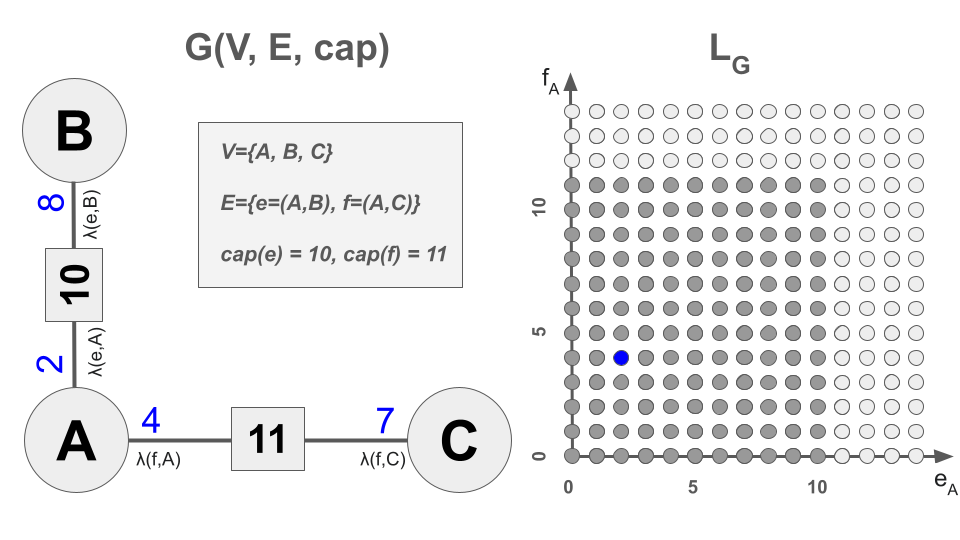
\includegraphics[width=0.35\textwidth]{StatepolytopeExample}}
%%     \subfigure[]{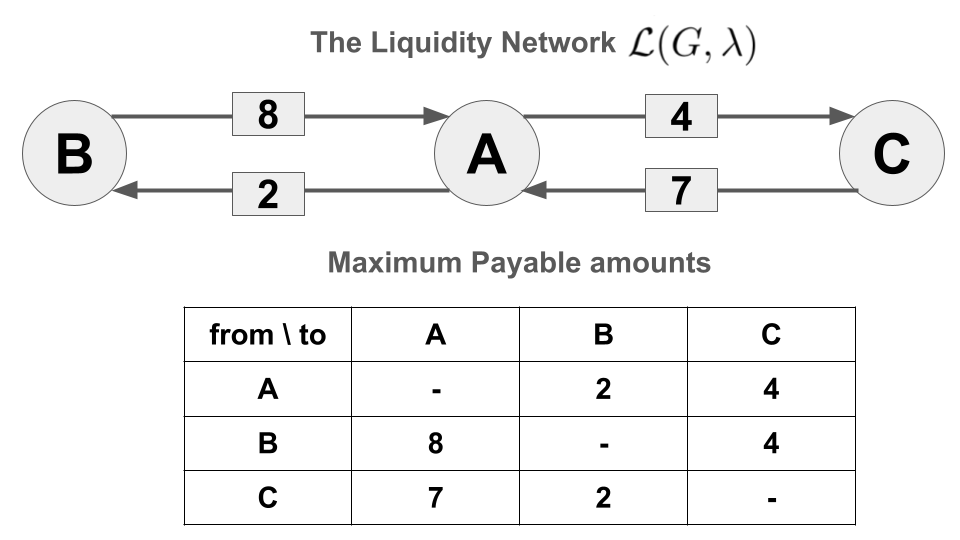
\includegraphics[width=0.35\textwidth]{liquidityNetwork}}
%% \caption{An Example Network $G$ with corresponding Polytope $L_G$ of liquidity states and liquidity network $\mathcal{L}(G,\lambda)$ for a fixed $\lambda\in L_G$} 
%% \end{figure}

%% For $2$-party channels (which are currently deployed on the Lightning Network) this is why knowing the liquidity of one peer is sufficient to know the entire state of the channel. 
%% Typically $e_v$ is only known to the peers $u,v$ that maintain the channel $e$.
%% Also the state $e_v$ can change over time as the node conducts payments or fulfills routing requests of other nodes.


\begin{definition}
For a fixed payment channel network \( G(V,E, \text{cap}) \), we define the set of all feasible liquidity functions, or the set of liquidity states of the network, as:
\[ L_G = \{\lambda: E \times V \longrightarrow \{0, \dots, C\} \mid \lambda(e,u) + \lambda(e,v) = \text{cap}(e) \}. \]
\end{definition}
This definition motivates the use of integer linear programming to examine \(L_G\) because the constraints are linear equations.
\begin{lemma}
The set \( L_G \) of all feasible liquidity states can be embedded into \(\mathbb{Z}^{2m}\).
\end{lemma}

\begin{proof}
Consider a basis \( \beta = \{ b_{e,x} \in \mathbb{Z}^{2m} \mid e \in E, x \in e \} \) where \( b_{e,x} \) are the \(2m\) basis vectors that span \(\mathbb{Z}^{2m}\). There is a natural embedding:
\[
\begin{aligned}
\iota: L_G & \longhookrightarrow \mathbb{Z}^{2m}, \\
\lambda & \stackrel{\iota}{\longmapsto} \sum_{e \in E, x \in e} e_x \cdot b_{e,x} \\
& = \sum_{e=(u,v) \in E} \left( e_u \cdot b_{e,u} + e_v \cdot b_{e,v} \right).
\end{aligned}
\]
\end{proof}

Let \( e_i = (u_i, v_i) \) be the \( i \)-th edge, then we can fix an order of \( \beta \) via:
\( \beta = \langle b_{e_1, u_1}, b_{e_1, v_1}, \dots, b_{e_m, u_m}, b_{e_m, v_m} \rangle. \)
In particular, we write:\( c_i = \text{cap}(e_i). \)

\begin{lemma}
\label{lem:dimensionOfStatePolytope}
The set \( L_G \) of feasible liquidity functions on a network \( G \) is isomorphic to an \( m \)-dimensional hyperbox \( H_G \subset \mathbb{Z}^{m} \). In particular:
\[ H_G = \{ 0, \dots, c_1 \} \times \dots \times \{ 0, \dots, c_m \}. \]
\end{lemma}
\begin{proof}
We prove this by showing that the forgetful function \( f: \iota(L_G) \longrightarrow H_G \) defined as
\[ \iota(\lambda) = \sum_{e=(u,v) \in E} \left( e_u \cdot b_{e,u} + e_v \cdot b_{e,v} \right) \stackrel{f}{\longmapsto} \sum_{e=(u,v) \in E} e_u \cdot b_{e,u} \]
is bijective. This involves showing that \( f \) is both injective and surjective.

\textbf{Injectivity}: Let \( \lambda \neq \mu \in L_G \). There must be at least one edge \( e=(u,v) \in E \) such that \( \lambda(e,u) \neq \mu(e,u) \). Consequently, by definition of \( f \), we have \( f(\iota(\lambda)) \neq f(\iota(\mu)) \). This is sufficient to show that \( f \) is injective.

\textbf{Surjectivity}: To show that \( f \) is surjective, take an arbitrary point \( x = (x_1, \dots, x_m) \in H \). We choose \( \lambda \) such that for all \( e_i \in E \):
\( \lambda(e_i, u_i) = x_i. \)
Because of the conservation of liquidity, we have:
\( \lambda(e_i, v_i) = \text{cap}(e_i) - \lambda(e_i, u_i) = c_i - x_i. \)
Since \( x_i \in \{0, \dots, c_i\} \), we can conclude that both \( \lambda(e_i, u_i) = x_i \) and \( \lambda(e_i, v_i) = c_i - x_i \) take values from \(\{0, \dots, c_i\}\). Thus, we have constructed \( \lambda \) such that \( f(\lambda) = x \), showing that \( f \) is also surjective.

This concludes our proof that \( f \) is bijective and that \( L_G \) is isomorphic to the \( m \)-dimensional hyperbox \( H_G \).
\end{proof}

We can see a low dimensional visualization of the introduced concepts in figure \ref{fig:statePolytopeExample}.

\begin{figure}[h]
  \centering
  \subfigure[]{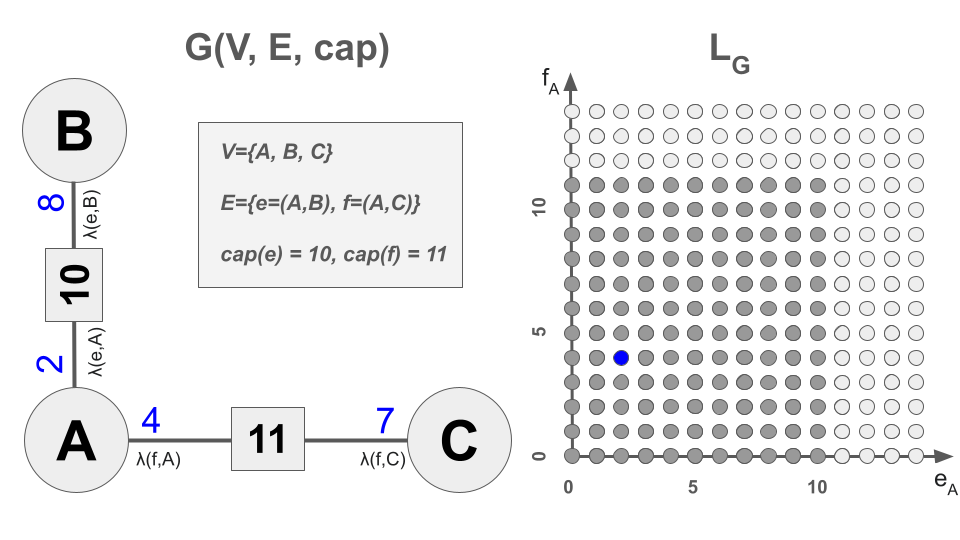
\includegraphics[width=0.38\textwidth]{StatepolytopeExample}}
  \subfigure[]{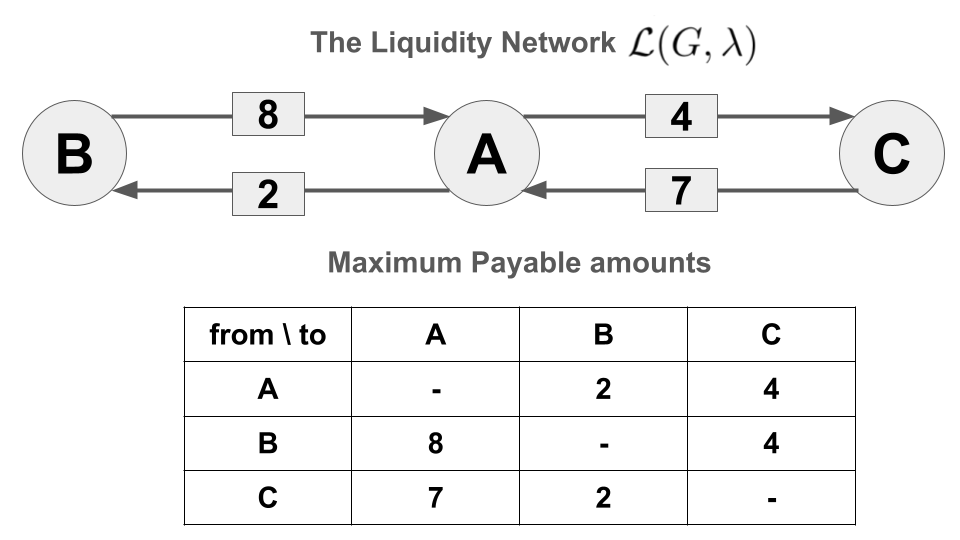
\includegraphics[width=0.38\textwidth]{liquidityNetwork}}
  \caption{An Example Network \( G \) with corresponding Polytope \( L_G \) of liquidity states and liquidity network \( \mathcal{L}(G,\lambda) \) for a fixed \( \lambda \in L_G \).}
  \label{fig:statePolytopeExample}
\end{figure}

For two-party channels, as currently deployed on the Lightning Network, knowing the liquidity of one peer is sufficient to determine the entire state of the channel. Typically, \( e_v \) is only known to the peers \( u \) and \( v \) who maintain the channel \( e \). The state \( e_v \) can change over time as the node conducts payments or fulfills routing requests from other nodes.

%https://math.stackexchange.com/questions/1517517/maximize-volume-of-hyperrectangle-given-fixed-sum-of-components
%https://math.stackexchange.com/questions/3074762/prove-than-cube-has-a-bigger-volume-than-cuboid-with-the-same-sum-of-edge-length
%% As a consequence of lemma \ref{lem:dimensionOfStatePolytope} the number of elements (aka network states) in $L_G$ is given by
%% $$vol(L_G):=|L_G| = \prod_{i=1}^m(c_i+1)$$
%% Assuming that the number of channels $m$ divides the total number of coins $C$ and as a consequence of the inequality of arithmetic and geometric means\cite{steele2004cauchy} one can see that the network in which all channels have the same capacity $\frac{C}{m}$ maximizes the volume of the corresponding polytope $L_G$ of Liquidity states.
%% In particular the maximum volume is given by $vol(S)=\left(\frac{C}{m}+1\right)^m$ and is depicted in figure \ref{fig:statePolytope}.

%% \begin{figure}[h]
%% \centering
%% 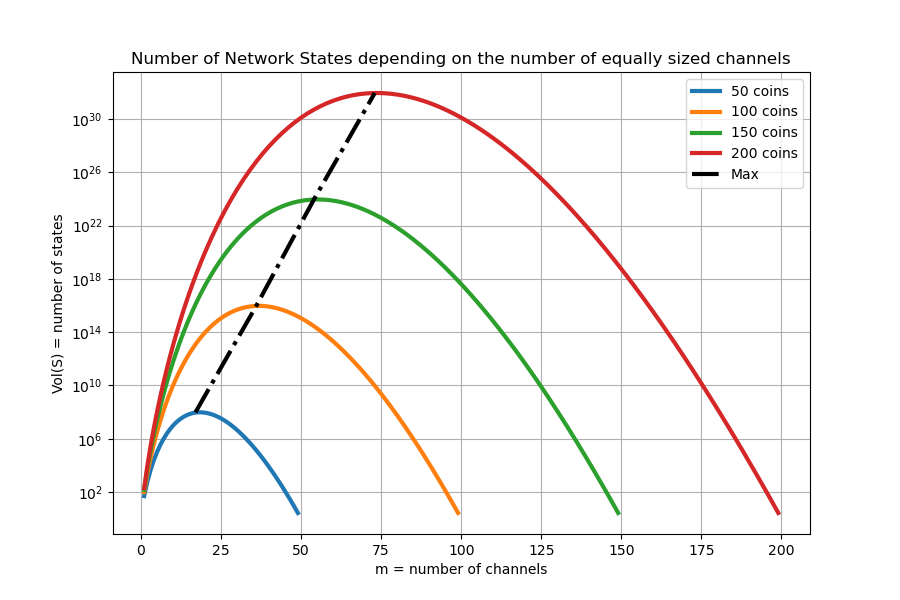
\includegraphics[width=0.5\textwidth]{size_of_state_polytope}
%% \caption{Volumes $vol(L_G)=\left(\frac{C}{m}+1\right)^m$ of state polytopes with equally sized channels for various number $C$ of coins and various number $m$ of channels.}
%% \label{fig:statePolytope}
%% \end{figure}

\begin{corollary}
The number of feasible network states is given by the volume of \( L_G \) which can be computed as:
\[ \text{vol}(L_G) := |L_G| = \prod_{i=1}^m (c_i + 1). \]
\end{corollary}

Assuming the number of channels \( m \) divides the total number of coins \( C \), and using the inequality of arithmetic and geometric means \cite{steele2004cauchy}, it can be shown that the network in which all channels have the same capacity \( \frac{C}{m} \) maximizes the volume of the corresponding polytope \( L_G \) of liquidity states. 
In particular, the maximum number of feasible network states is given by:
\[ \text{vol}(L_G) = \left( \frac{C}{m} + 1 \right)^m, \]
and is depicted in figure \ref{fig:statePolytope} for various number of coins and channels.

\begin{figure}[h]
\centering
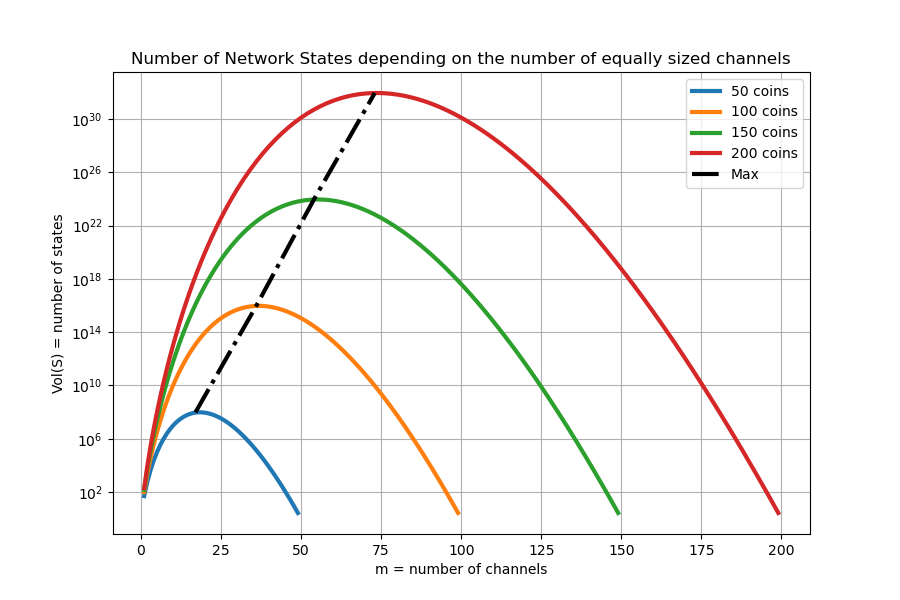
\includegraphics[width=0.5\textwidth]{size_of_state_polytope}
\caption{Volumes \( \text{vol}(L_G) = \left( \frac{C}{m} + 1 \right)^m \) of state polytopes with equally sized channels for various numbers \( C \) of coins and various numbers \( m \) of channels.}
\label{fig:statePolytope}
\end{figure}

\section{Polytope of feasible Wealth Distributions}
%% So far we have focused on the liquidity states of payment channel networks.
%% From the perspective of a user we may be more interested in the wealth of the user instead of how the wealth is specifically allocated to the channels. 
%% We make a short intermezzo to study the onchain situation before showing how payment channel networks put additional constraints to the polytope of feasible wealth distributions of the users. 
%% \begin{definition}
%% Let $V = \{v_1,\dots,v_n\}$ be the set of $n$ Bitcoin users who own in total $C$ coins.
%% We call a function $\omega:V\longrightarrow\mathbb{N}_0$ a wealth distribution if and only if $C = \sum_{i=1}^n\omega(v_i)$.
%% We call
%% $$W(C,n)=\{\omega:V\longrightarrow \mathbb{N}_0 | C = \sum_{i=1}^n\omega(v_i)\}$$
%% the set of Bitcoin wealth distributions.
%% \end{definition}

%% We use the same methodology as with liquidity functions to show that $W(C,n)$ is isomorph to the Polytope $\mathcal{W}(C,n)$ that one gets by intersecting the $n$ half spaces defined as $\mathbb{Z}_i=\{x\in\mathbb{Z}^n|x_i\geq 0\}$ with the $n-1$ dimensional hyperplane $P_C$ defined by the linear equation:
%% $$P(C,n)=\{w\in\mathbb{Z}^n | w_1 + \dots + w_n = C\}$$
%% In particular:
%% $$\mathcal{W}(C,n) = P(C,n)\cap\left(\bigcap_{i=1}^n\mathbb{Z}_i\right)$$
%% In order to do so we chose a base $\beta = \{b_{v} \in \mathbb{Z}^{n}| v\in V\}$ with $b_{v}$ being the $n$ base vectors that span $\mathbb{Z}^{n}$.
%% Similar to the situation with liquidity functions there is a natural embedding:

We have focused on the liquidity states of payment channel networks so far. However, from a user's perspective, their overall wealth might be of more interest than how this wealth is allocated across different channels. Before exploring how payment channel networks impose additional constraints on the polytope of feasible wealth distributions, we will briefly examine the on-chain situation.

\begin{definition}
Let \( V = \{v_1, \dots, v_n\} \) be the set of \( n \) Bitcoin users who collectively own \( C \) coins. We define a function \( \omega: V \longrightarrow \mathbb{N}_0 \) as a wealth distribution if and only if \( C = \sum_{i=1}^n \omega(v_i) \). We denote the set of Bitcoin wealth distributions as
$$
W(C,n) = \{\omega: V \longrightarrow \mathbb{N}_0 \mid C = \sum_{i=1}^n \omega(v_i)\}.
$$
\end{definition}

We use the same methodology as with liquidity functions to show that \( W(C,n) \) is isomorphic to the polytope \( \mathcal{W}(C,n) \), which is obtained by intersecting the \( n \) half-spaces \( \mathbb{Z}_i = \{x \in \mathbb{Z}^n \mid x_i \geq 0\} \) with the \( n-1 \) dimensional hyperplane \( P_C \) defined by the linear equation:
$$
P(C,n) = \{w \in \mathbb{Z}^n \mid w_1 + \dots + w_n = C\}.
$$
Specifically,
$$
\mathcal{W}(C,n) = P(C,n) \cap \left( \bigcap_{i=1}^n \mathbb{Z}_i \right).
$$

To demonstrate this, we choose a basis \( \beta = \{b_{v} \in \mathbb{Z}^{n} \mid v \in V\} \) with \( b_{u} \) being the \( n \) base vectors that span \( \mathbb{Z}^{n} \). Similar to the case with liquidity functions, there is a natural embedding:

\begin{equation*}
  \begin{split}
\iota: W(C,n) \longhookrightarrow & \mathbb{Z}^{n} \\
\omega\stackrel{\iota}{\longmapsto} & \sum_{v\in V}\omega(v)\cdot b_{v}
\end{split}
\end{equation*}

\begin{lemma}
  The image of $\iota$ is $\mathcal{W}(C,n)$.
\end{lemma}
\begin{proof}
  Let $w\in \mathcal{W}(C,n)$ with
  $$w = \sum_{i=1}^nw_i\cdot b_{u_i}$$
  We select $\omega\in W(C,n)$ such that $\omega(v_i)=w_i$
  This is the preimage of $\iota^{-1}(w)$.
  If $w'\in \mathbb{Z}^n\backslash\mathcal{W}(C,n)$ then no $\omega$ with $\iota(\omega)=w'$ exists.
\end{proof}

%% Because of the embedding we might in future refer to wealth distributions as wealth vectors.
%% From the lemma and the stars and bars theorem\footnote{\url{https://en.wikipedia.org/wiki/Stars_and_bars_(combinatorics)}} it follows that the number $|\mathcal{W}(C,n)|$ of wealth distributions of $n$ users with a fixed number of total of coins $C$ is

%% \begin{equation}
%% vol(\mathcal{W}(C,n):=|\mathcal{W}(C,n)| = {{C + n - 1}\choose {n - 1}}
%% \end{equation}

%% For example assume the $n=3$ users Alice, Bob and Carol have $C=21$ coins that they wish to split among themselves.
%% They would have a total of $253$ ways to do so.
%% Those can be observed in the $2$-dimensional polytope:
%% \begin{figure}[h]

%% \centering
%% 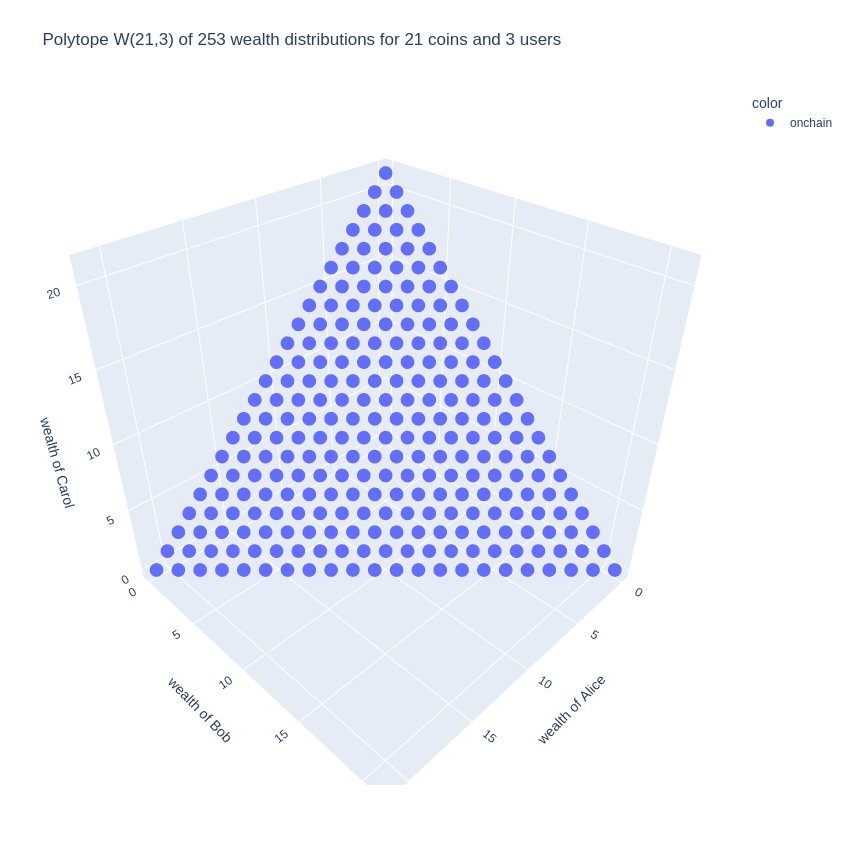
\includegraphics[width=0.5\textwidth]{polytope_of_bitcoin_wealth_distributions}
%% \caption{$3$-dimensional embedding of the $2$-dimensional polytope of wealth distributions of $C=21$ coins among $n=3$ users.} 
%% \label{fig:wealthPolytope}
%% \end{figure}

%% Knowing the volume of the polytope of feasible bitcoin wealth distributions will serve as reference point when studying the feasible wealth distributions $W_G$ in a payment channel network $G$. 

Because of the embedding, we may refer to wealth distributions as wealth vectors. From the lemma and the stars and bars theorem\footnote{\url{https://en.wikipedia.org/wiki/Stars_and_bars_(combinatorics)}}, it follows that the number \( |\mathcal{W}(C,n)| \) of wealth distributions for \( n \) users with a fixed total of \( C \) coins is given by:

\begin{equation}
\text{vol}(\mathcal{W}(C,n)) := |\mathcal{W}(C,n)| = \binom{C + n - 1}{n - 1}
\end{equation}

For example, assume the \( n=3 \) users Alice, Bob, and Carol have \( C=21 \) coins to distribute among themselves. They would have a total of \( 253 \) ways to do so. These distributions can be represented in a \( 2 \)-dimensional polytope:

\begin{figure}[h]
\centering
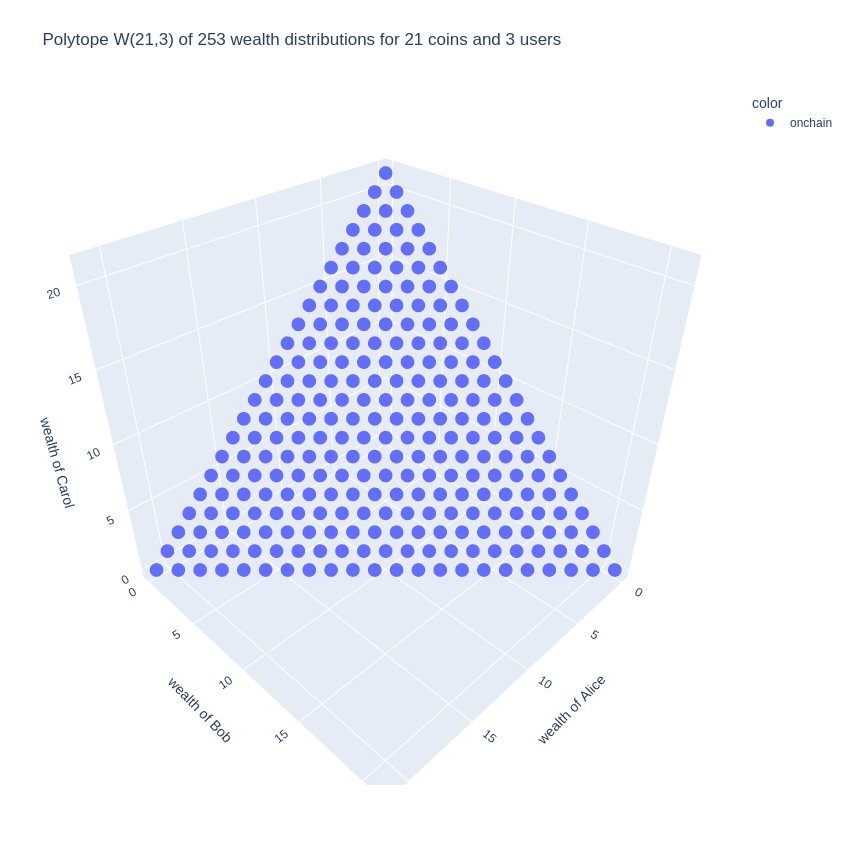
\includegraphics[width=0.5\textwidth]{polytope_of_bitcoin_wealth_distributions}
\caption{$3$-dimensional embedding of the $2$-dimensional polytope of wealth distributions of $C=21$ coins among $n=3$ users.}
\label{fig:wealthPolytope}
\end{figure}

Knowing the volume of the polytope of feasible Bitcoin wealth distributions will serve as a reference value when studying the feasible wealth distributions \( W_G \) in a payment channel network \( G \).

\subsection{The Polytope $W_G$ of feasible Wealth Distributions of a Payment Channel Network $G$}
%% Instead of looking at all wealth distributions of $C$ coins between $n$ users we are just interested in those that are feasible on a given payment channel neetwork $G(V,E,cap)$.
%% \begin{definition}
%%   Given a payment channel network $G(V,E,cap)$ with $|V|=n$ users and $C$ coins. We call a wealth distribution: $\omega: V\longrightarrow \{0,\dots,C\}$ feasible in $G$ if there exists a liquidity function $\lambda$ such that for all $v\in V$:
%%   \begin{equation}
%%   \sum_{e\in E: v\in e}\lambda(e,v)=\omega(v)
%%   \end{equation}
%%   In particular we call:
%%   $$\{\omega \in W(C,n)|\exists \lambda\in L_G: \sum_{e\in E: v\in e}\lambda(e,v)=\omega(v) \forall v\in V\}$$
%%   the set $W_G$ of wealth distributions that are feasible in $G$.  
%% \end{definition}

%% We will now study how conservation of liquidity in payment channels reduces the volume of feasible wealth distributions $W_G$ for a given payment channel network.

%% \begin{lemma}
%%   \label{lem:subset}
%%   Let $G(V,E,cap)$ be a payment channel network.
%% For $n>2$ there exists $\omega\in W(C,n)$ such that $\omega\not\in W_G$. 
%% \end{lemma}
%% \begin{proof}
%%   We proof this by contradiction.
%%   Let $e=(u,v)\in E$ be an arbitrary channel with capacity $c_{e}>0$.
%%   Because $n>2$ there is a user $w$ with $u\neq w\neq v$.
%%   We set $\omega:V\longrightarrow \mathbb{N}$ as:
%%     \begin{equation}
%%     \omega(x)= \begin{cases}
%%       C & \text{if $x=w$}\\
%%       0 & \text{otherwise}
%%     \end{cases}
%%     \end{equation}
%%     By construction we have $C=\sum_{x\in V}\omega(x)$.
%%     Thus $\omega$ is feasible in $W(C,n)$.
%%     In particular $\omega(u)=\omega(v)=0$.

%%     To conclude the proof we assume $\omega\in W_G$.
%%     Then due to conservation of liquidity (equation \ref{eq:conservationOfLiquidity}) and by definition of $\omega$ being a feasible wealth functions in $G$ we know that $\omega(u) + \omega(v) \geq c_{e}$.
%%   This contraticts the assumption that the capacity of the channel was non $0$. 
%% \end{proof}

Instead of examining all wealth distributions of \( C \) coins among \( n \) users, we focus on those distributions that are feasible within a given payment channel network \( G(V,E,cap) \).

\begin{definition}
Given a payment channel network \( G(V,E,cap) \) with \( |V|=n \) users and \( C \) coins, a wealth distribution \( \omega: V \longrightarrow \{0,\dots,C\} \) is called feasible in \( G \) if there exists a liquidity function \( \lambda \) such that for all \( v \in V \):
\begin{equation}
\sum_{e \in E: v \in e} \lambda(e,v) = \omega(v)
\end{equation}
We denote the set of wealth distributions that are feasible in \( G \) as:
$$\{\omega \in W(C,n) | \exists \lambda \in L_G: \sum_{e \in E: v \in e} \lambda(e,v) = \omega(v) \forall v \in V\}$$
This set is referred to as \( W_G \).
\end{definition}

Next, we will study how the conservation of liquidity in payment channels reduces the volume of feasible wealth distributions \( W_G \) for a given payment channel network.

\begin{lemma}
\label{lem:subset}
Let \( G(V,E,cap) \) be a payment channel network. For \( n > 2 \), there exists \( \omega \in W(C,n) \) such that \( \omega \notin W_G \).
\end{lemma}

\begin{proof}
We prove this by contradiction. Let \( e = (u,v) \in E \) be an arbitrary channel with capacity \( c_e > 0 \). Since \( n > 2 \), there is a user \( w \) such that \( u \neq w \neq v \). We define \( \omega: V \longrightarrow \mathbb{N} \) as:

\begin{equation}
\omega(x) = \begin{cases}
C & \text{if } x = w \\
0 & \text{otherwise}
\end{cases}
\end{equation}

By construction, we have \( C = \sum_{x \in V} \omega(x) \). Thus, \( \omega \) is feasible in \( W(C,n) \), and specifically, \( \omega(u) = \omega(v) = 0 \).

To conclude the proof, assume \( \omega \in W_G \). Due to the conservation of liquidity (equation \ref{eq:conservationOfLiquidity}) and the definition of \( \omega \) as a feasible wealth function in \( G \), we know that \( \omega(u) + \omega(v) \geq c_e \). This contradicts the assumption that the capacity of the channel was non-zero.
\end{proof}


%% \begin{corollary}
%% The number $|W|$ of feasibile wealth distributions of $C$ coins between $n>2$ users in a payment channel network is strictly smaller than the number $|W_C|$ of wealth distributions that are feasible with on chain transactions.  
%% \end{corollary}

%% We will be interested how the topology of $G$ impacts the relative volume $r(G)$ that $W_G$ has in comparison to $\mathcal{W}(C,n)$ 
%% \begin{equation}
%%   r(G) = \frac{|W_G|}{|\mathcal{W}(C,n)|}
%% \label{eq:relVolume}
%% \end{equation}

%% For example if we take the network from the last section in figure \ref{fig:statePolytopeExample} we can observe the feasible region $W_G$ as a subpolytope of $\mathcal{W}(21,3)$ in figure \ref{fig:wealthPolytope}
%% \begin{figure}[h]
%%   \label{fig:wealthPolytope}
%% \centering
%% \includegraphics[width=0.5\textwidth]{polytope_of_wealth_distributions_inequal}
%% \caption{Only $52.17\%$ of all wealth distributions of $\mathcal{W}(21,3)$ are feasible if Alice Bob and Carol allocate the $21$ coins into $2$ channels of capacity $10$ and $11$.} 
%% \end{figure}

%% We are not aware of an alytically closed formula that describes the volume $|W_G|$ for a given network $G$. 
%% However we can estimate the volume throgh statistical sampling via Monte Carlo methods.
%% Utilizing the Dirichlet Rescale Algorithm\cite{griffin2020generating} we are able to uniformly randomly select wealth distributions $\omega$ from $\mathcal{W}(C,n)$.\footnote{an open source implementation can be found at: \url{https://github.com/dgdguk/drs}}
%% We can then check how often they are feasible for a given network $G$.
%% This gives us an estimate for $r(G)$:
%% \begin{equation}
%%   r(G)\approx \frac{\text{number of $\omega$ such that $\omega$ is feasible in $G$}}{\text{number of sampled $\omega\in\mathcal{W}(C,n)$}}
%% \end{equation}

\begin{corollary}
The number \( |W_G| \) of feasible wealth distributions of \( C \) coins among \( n > 2 \) users in a payment channel network is strictly smaller than the number \( |\mathcal{W}(C,n)| \) of wealth distributions that are feasible with on-chain transactions.
\end{corollary}

We are interested in how the topology of \( G \) impacts the relative volume \( r(G) \) that \( W_G \) has in comparison to \( \mathcal{W}(C,n) \):

\begin{equation}
r(G) = \frac{|W_G|}{|\mathcal{W}(C,n)|}
\label{eq:relVolume}
\end{equation}

For example, consider the network from the previous section in Figure \ref{fig:statePolytopeExample}. We can observe the feasible region \( W_G \) as a subpolytope of \( \mathcal{W}(21,3) \) in Figure \ref{fig:wealthPolytope}.

\begin{figure}[h]
\centering
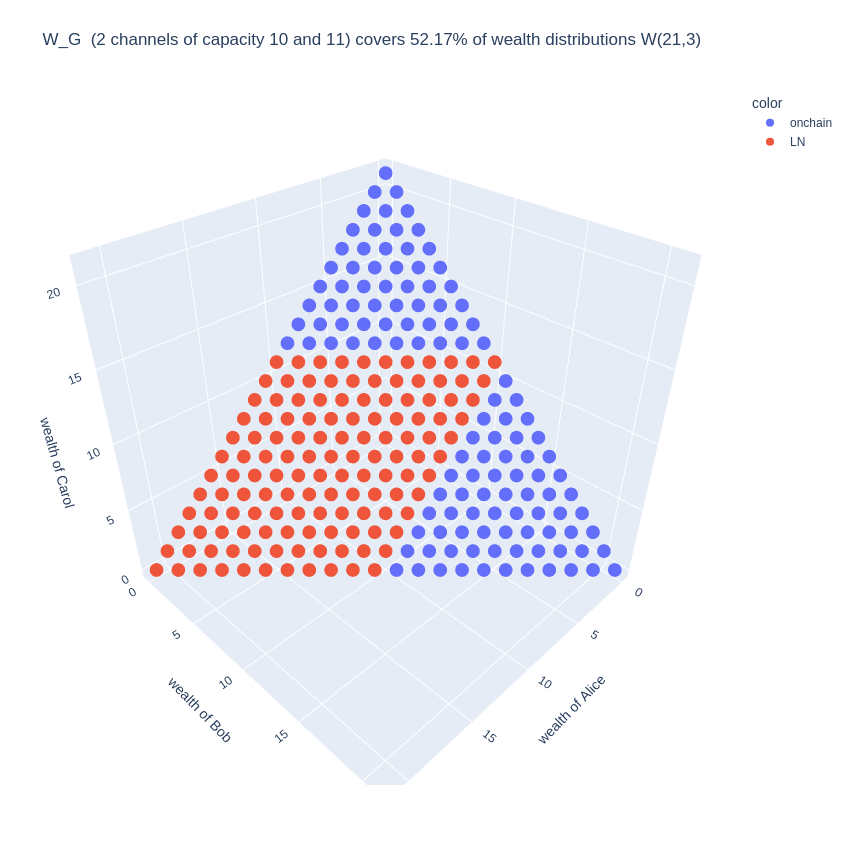
\includegraphics[width=0.5\textwidth]{polytope_of_wealth_distributions_with_ln}
\caption{Only 52.17\% of all wealth distributions in \( \mathcal{W}(21,3) \) are feasible if Alice, Bob, and Carol allocate the 21 coins into 2 channels of capacities 10 and 11.}
\label{fig:wealthPolytope}
\end{figure}

We Note that the feasible reagion changes with the topology of the network.
If Bob Spliced out 7 coins of his channel with Alice and created a new channel of 7 coins the feasible reagion would increase in size as can be seen in figure \ref{fig:feasibleLNWealthPolytopes}(a).
However the increase is relatively small.
It becomes larger if all channels had the same capcity as can be seen in figure \ref{fig:feasibleLNWealthPolytopes} (b).

\begin{figure}[h]
  \centering
  \subfigure[]{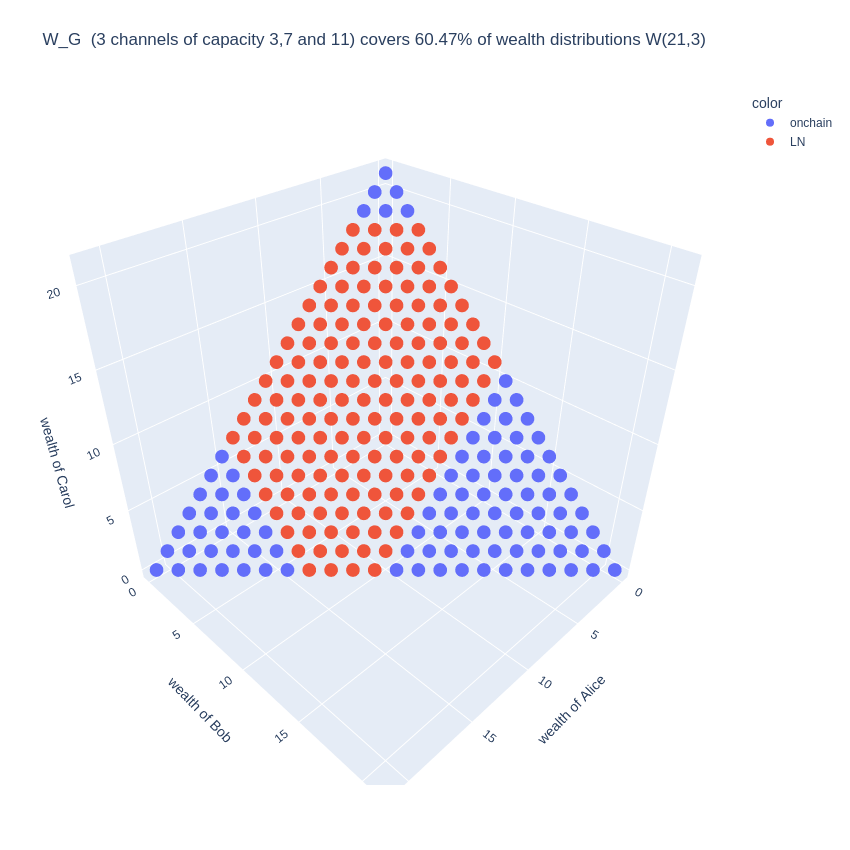
\includegraphics[width=0.23\textwidth]{polytope_of_wealth_distributions_lninequal}}
  \subfigure[]{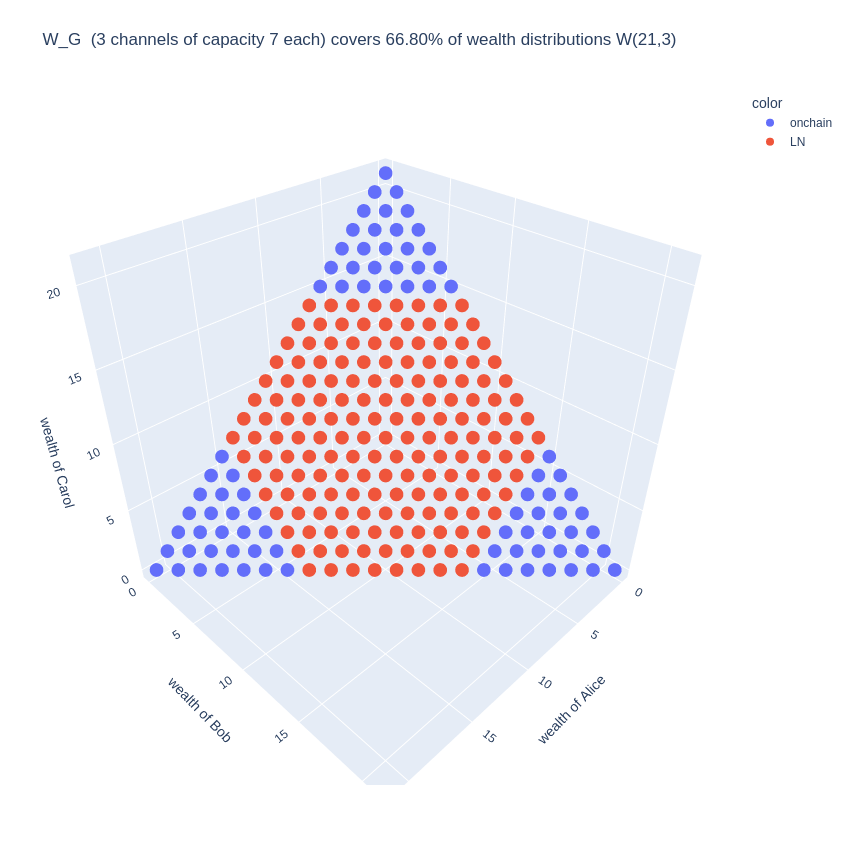
\includegraphics[width=0.23\textwidth]{polytope_of_wealth_distributions_lnequal}}
  \caption{$2$ feasible regions of $W_G$ for $2$ different networks between Alice Bob and Carol who own in total $21$ coins.}
  \label{fig:feasibleLNWealthPolytopes}
\end{figure}


We are not aware of an analytically closed formula that describes the volume \( |W_G| \) for a given network \( G \).
In particular we are not aware of a smart way to find the topology $G$ that maximizes $r(G)$.
However, we can estimate the volume through statistical sampling via Monte Carlo methods. Utilizing the Dirichlet Rescale Algorithm \cite{griffin2020generating}, we can uniformly and randomly select wealth distributions \( \omega \) from \( \mathcal{W}(C,n) \).\footnote{An open source implementation can be found at: \url{https://github.com/dgdguk/drs}} We can then check how often these distributions are feasible for a given network \( G \). This gives us an estimate for \( r(G) \):
\begin{equation}
r(G) \approx \frac{\text{number of \( \omega \) such that \( \omega \) is feasible in \( G \)}}{\text{number of sampled \( \omega \in \mathcal{W}(C,n) \)}}
\end{equation}
In order to be able to evaluate this we need to be able to decide if a given wealth distribution in $\mathcal{W}(C,n)$ is feasible in $W_G$.

\subsection{Deciding if a Wealth Distribution $\omega\in\mathcal{W}(C,n)$ is also feasible in $W_G$}
\label{sec:isomorphism}
%% Due to lemma \ref{lem:subset} we know there exists at least one vector $\omega\in \mathcal{W}(C,n)$ that is infeasible and not in $W_G$.
%% For an arbitrary vector $\omega\in \mathcal{W}(C,n)$ we can decide if it is also an Element of $W_G$ and thus a feasible welth distribution on the payment channel network.
%% According to the definition of being a feasible wealth distribution in $W_G$ we need to provide $\lambda\in L_G$ such that $\forall e \in E, v\in V$ the following $n$ linear equations hold:
%% \begin{equation}
%%   \label{eq:wealthConstraints}
%%   \sum_{e\in E: v\in e}\lambda(e,v)=\omega(v)
%%   \end{equation}
%%   Because of conservation of liquidity $\lambda$ requires an additional $m$ equations $\forall e\in E$:
%%   \begin{equation}
%%     \label{eq:channelConstraints}
%%     \lambda(e,v)+\lambda(e,u)=cap(e)
%%   \end{equation}
%%   Thus we need to solve a system of $n+m$ linear equations in $2\cdot m$ variables:
%%   $$\{e_{1,{u_1}},e_{1,v_1},\dots,e_{m,u_m},e_{m,v_m}\}$$
%%   Those equations are not fully independent because summing up the $n$ equations from equation \ref{eq:wealthConstraints} we get the same value as summing up the $m$ equations from equation \ref{eq:channelConstraints}:
%%   $$\sum_{v\in V}\sum_{e\in E: v\in e}\lambda(e,v) = C = \sum_{e=(u,v)\in E}\left(\lambda(e,v)+\lambda(e,u)\right)$$
%%   Therefor we can eliminate one of the constraints and have in total only $m+n-1$ independent equations.
%%   Let $\sigma(G,\omega)$ be the solution space of feasible liquidity functions on $G$ for the the above system of linear equations over intergers. 
%%   If solved over $\mathbb{Z}^{2\cdot m}$ the space $\sigma(G,\omega)$ is at least $2\cdot m-(m+n-1)=(m-n+1)$-dimensional.
%%   However we are seeking solutions over $L_G$ which is isomorph to the bounded hypercube:
%%   $$H_G=\{0,\dots,c_1\}\times\{0,\dots,c_m\}$$
%%   Thus for a wealth distribution to be feasible and a liquidity function $\lambda$ to exist we must require:
%%   \begin{equation}
%%     \sigma(G,\omega)\cap H_G \neq\emptyset
%%   \end{equation}
%%   Finding a solution for the system of linear equations over intergers in a bounded region can be done through integer linear programming.\footnote{As discussed with Stefan Richter. Instead of solving a system of linear equations over a bounded region one could solve a max flow problem to test feasibility. For this one would take an arbitrary wealth vector $w'$ and compute $w-w'´$. The components of the difference are the supply and demand of the nodes in the network. If a multi source multi sink flow exists that fulfills the supply and demand then $w\in W_G$}

Due to Lemma \ref{lem:subset}, we know there exists at least one vector \( \omega \in \mathcal{W}(C,n) \) that is infeasible and not in \( W_G \).  
For an arbitrary vector \( \omega \in \mathcal{W}(C,n) \), we can determine if it is also an element of \( W_G \) and thus a feasible wealth distribution on the payment channel network.  
According to the definition of a feasible wealth distribution in \( W_G \), we need to find \( \lambda \in L_G \) such that for all \( e \in E \) and \( v \in V \), the following \( n \) linear equations hold:  
\begin{equation}
  \label{eq:wealthConstraints}
  \sum_{e \in E: v \in e}\lambda(e,v) = \omega(v)
\end{equation}
Due to the conservation of liquidity, \( \lambda \) requires an additional \( m \) equations for all \( e \in E \):  
\begin{equation}
  \label{eq:channelConstraints}
  \lambda(e,v) + \lambda(e,u) = \text{cap}(e)
\end{equation}
Thus, we need to solve a system of \( n + m \) linear equations in \( 2 \cdot m \) variables:  
\[ \{e_{1,{u_1}}, e_{1,v_1}, \dots, e_{m,u_m}, e_{m,v_m} \} \]  
These equations are not fully independent because summing the \( n \) equations from Equation \ref{eq:wealthConstraints} yields the same value as summing the \( m \) equations from Equation \ref{eq:channelConstraints}:  
\[ \sum_{v \in V}\sum_{e \in E: v \in e}\lambda(e,v) = C = \sum_{e=(u,v) \in E}\left(\lambda(e,v) + \lambda(e,u)\right) \]  
Therefore, we can eliminate one of the constraints, resulting in a total of \( m + n - 1 \) independent equations.  
Let \( \sigma(G,\omega) \) be the solution space of feasible liquidity functions on \( G \) for the above system of linear equations over integers.  
If solved over \( \mathbb{Z}^{2 \cdot m} \), the dimension of the solution space \( \sigma(G,\omega) \) is at least \( 2 \cdot m - (m + n - 1) = (m - n + 1) \). 
However, we are seeking solutions over \( L_G \), which is isomorphic to the bounded hypercube:  
\[ H_G = \{0, \dots, c_1\} \times \{0, \dots, c_m\} \]  
Thus, for a wealth distribution to be feasible and a liquidity function \( \lambda \) to exist, we must require:  
\begin{equation}
  \sigma(G,\omega) \cap H_G \neq \emptyset
\end{equation}
Finding a solution for the system of linear equations over integers in a bounded region can be done through integer linear programming.  
\footnote{As discussed with Stefan Richter. Instead of solving a system of linear equations over a bounded region, one could solve a max flow problem to test feasibility. For this, one would take an arbitrary wealth vector \( \omega' \) and compute \( \omega - \omega' \). The components of the difference are the supply and demand of the nodes in the network. If a multi-source, multi-sink flow exists that fulfills the supply and demand, then \( \omega \in W_G \).}


\subsubsection{A Remark on Credit in Payment Channel Networks}
The previous geometric example illustrates that the system of linear equations that come from conservation of liquidity and the network topology always has at least one solution over $\mathbb{Z}^{2\cdot m}$.
However if the intersection of the solution space \(\sigma(G,\omega) \cap H_G\) is empty this means that all elements of $\sigma(G,\omega)$ have at least once component that is negative. 
This shows that some wealth distributions are infeasible on payment channel networks because the liquidity of the peers in the channel has to be always positive.
If credit was allowed in channels a feasible network state could be constructed for any wealth distribution.
A similar result has been shown before the Lightning Network was created \cite{dandekar2011liquidity}
Of course credit requirs trust and is consequently not wished for by the users and developers of peer to peer electronic payment systems.
However this geometric insight shows how difficult it is to create trustless electronic payment systems.


\subsection{Application: Deciding the Feasibility of Payments}
%% Making a payment is the same as changing the wealth vector.
%% Let us assume $w=(w_1,\dots,w_n)\in W_G$ is the current wealth distribution of the network.
%% If the $i$-th user wishes to pay user $j$ the amount $a$ we can test the feasibility of the payment by checking if
%% \begin{equation}
%%   \label{eq:payment}
%% w' = w + a\cdot b_j - a\cdot b_i
%% \end{equation}
%% is still inside the polytope $W_G$ of feasible wealth distributions.
%% If $w'\not\in W_G$ then given our initial wealth distribution $w$ the payment between $i$ and $j$ of amount $a$ will fail.

%% In particular because of lemma \ref{lem:subset}  payments between users may be infeasible within the payment channel network.
%% Importantly we note that in payment channel networks it is impossible that 100\% of all thinkable payment requests are feasible!

%% Quite remarkably, deciding weather a payment is feasible in a given network without conducting additional on chain operations does not depend on the exact state of the network.
%% Instead feasibility of a payment does only depend on the network topology and the current wealth distribution.
%% In particular the payment of amount $a$ between user $i$ and $j$ can be feasible or infeasible, depending on the current wealth distribution.
%% Of course similar to the liquidity state of the network the current wealth distribution is unkown.

%% Similarly to estimating $r(G)$ we can estimate the the likelihood that a payment is feasible through Monte Carlo methods.
%% For this we uniformly randomly sample several feasible wealth distributions in $W_G$ and compute how often the adopted distribution that we receive after executing the payment is feasible.
%% This method has already been shared in public before this paper was published.\footnote{\url{https://delvingbitcoin.org/t/estimating-likelihood-for-lightning-payments-to-be-in-feasible/973}}
%% It can help node operators in their decision making about opening or closing channels. 
%% Before we investige the relation between the polytope of liquidity states and the polytope of feasible wealth distributions we will illustrate our current understanding through a low dimensional example. 

Making a payment is equivalent to changing the wealth vector.  
Let us assume \( w = (w_1, \dots, w_n) \in W_G \) is the current wealth distribution of the network.  
If the \( i \)-th user wishes to pay user \( j \) the amount \( a \), we can test the feasibility of the payment by checking if  
\begin{equation}
  \label{eq:payment}
  w' = w + a \cdot b_j - a \cdot b_i
\end{equation}
is still inside the polytope \( W_G \) of feasible wealth distributions.  
If \( w' \notin W_G \), then given our initial wealth distribution \( w \), the payment between \( i \) and \( j \) of amount \( a \) will fail.  

Remarkably, deciding whether a payment is feasible in a given network without conducting additional on-chain operations does not depend on the exact state of the network.  
Instead, the feasibility of a payment depends only on the network topology and the current wealth distribution.  
Of course, similar to the liquidity state of the network, the current wealth distribution is unknown. 

Thus we take a global perspective.
Similarly to estimating \( r(G) \), we can estimate the likelihood that a payment is feasible through Monte Carlo methods.
For this, we uniformly randomly sample several feasible wealth distributions in \( W_G \) and compute how often the resultant distribution after executing the payment is feasible.\footnote{This method has already been shared publicly before this paper was published.\url{https://delvingbitcoin.org/t/estimating-likelihood-for-lightning-payments-to-be-in-feasible/973}}
Node operators can use this to decide where to allocate liquidity an which channels to open or close.  

\begin{definition}
  We call $\rho$ the expected rate of infeasible payments.
\end{definition}

In particular, due to Lemma \ref{lem:subset}, it is noted that in payment channel networks, it is impossible for 100\% of all conceivable payment requests to be feasible.  

\begin{figure}[h]
\centering
 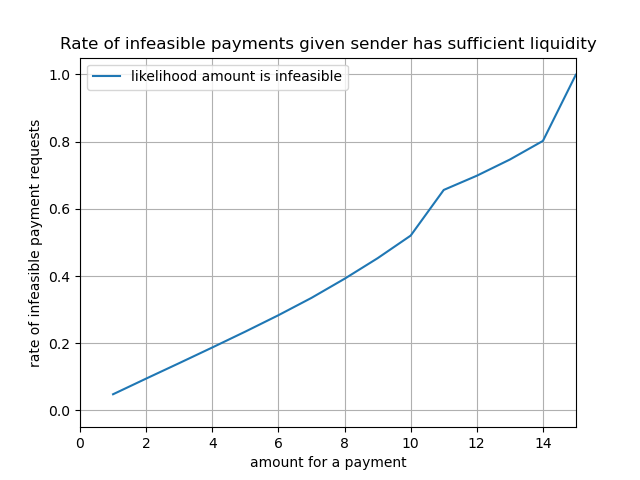
\includegraphics[width=0.40\textwidth]{rateofinfeasible}

\caption{Expected Rate \(\rho\) of infeasible payments in the example network between Alice, Bob, and Carol with channels of sizes 3, 7, and 11}
\label{fig:infeasible}
\end{figure}



\subsection{Limited Ability of Payment Channel Networks to scale Blockchains}
%% We emphasize that infeasible payment requests need at least one on chain transaction to be executed successfully.
%% This transaction can be used to  either change the wealth distribution and state of the payment channel network via an onchain / offchain swapping service or in order to change the topology of the network by opening an closing channels or through splicing.
%% If $\rho$ is the rate of expected infeasible payments and $\zeta$ the number of possible onchain transactions per second then we can derive the maximum bandwidth of supported lightning network payments as:
%% \begin{equation}
%% \text{supported payments per second} = \mathcal{S}  = \frac{\zeta}{\rho}
%% \end{equation}
%% In the Lightning Network whitepaper \cite{poon2016bitcoin} the authors state that the Visa Network supports $47'000$ payments per second in peak time.
%% Solving the equation for $\rho$ and noting that the Bitcoin network allows $\zeta=7$ tx/sec we conclude that only $\rho = \frac{7}{47´000} \sim 0.0149\%$ of all conceivable payments are allowed to be infeasible. 
%% Thus for payment channel networks to be able to scale the payment throughput of blockchains it is crucial that the rate $\rho$ of infeasible payments is close to zero.
%% This happens when the feasible reagion of wealth distributions $W_G$ is large within $W(C,n)$ or if $r(G)$ is close to $1$.

%% \begin{figure}[h]
%% \centering
%%  \subfigure[]{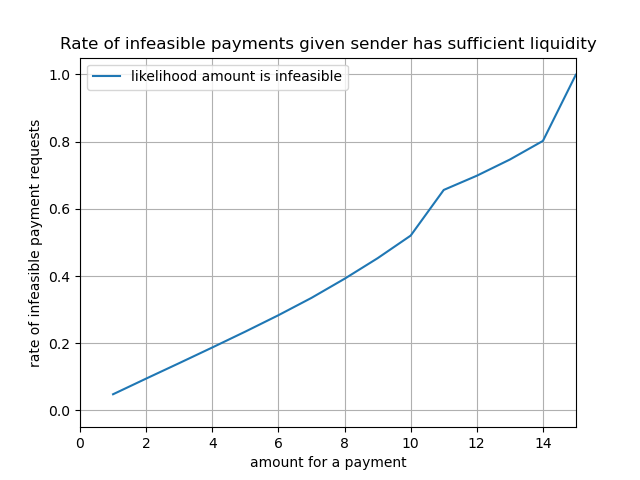
\includegraphics[width=0.23\textwidth]{rateofinfeasible}}
%%      \subfigure[]{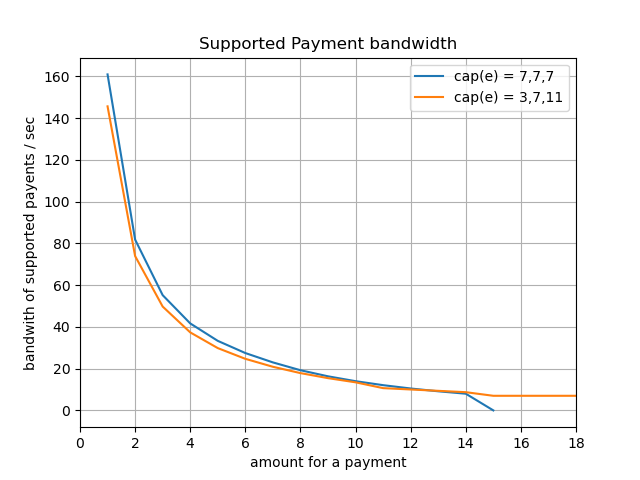
\includegraphics[width=0.23\textwidth]{paymentrate}}

%% \caption{Rate of infeasible payments $\rho$ depending on the desired payment amount $a$ on the example network between Alice, Bob and Carol with channels of Size $3,7$ and $11$}
%% \label{fig:infeasible}
%% \end{figure}
%% In the afore mentioned blog article we have shared a figure similar to \ref{fig:infeasible}. This demonstrates that already on our tiny example network the rate $\rho$ of infeasible payments is higher than $1\%$.
%% We will see later in this document that with larger $2$ party channel networks the relative volume $r(G)$ declines. 

We emphasize that infeasible payment requests require at least one on-chain transaction to be executed successfully.  
This transaction can either change the wealth distribution and state of the payment channel network via an on-chain/off-chain swapping service or alter the network topology by opening and closing channels or through splicing.  
If \( \zeta \) is the number of possible on-chain transactions per second, we can derive the maximum bandwidth of supported Lightning Network payments as:  
\begin{equation}
\text{supported payments per second} = \mathcal{S} = \frac{\zeta}{\rho}
\end{equation}

In the Lightning Network whitepaper \cite{poon2016bitcoin}, the authors state that the Visa Network supports 47,000 payments per second during peak times.  
Solving the equation for \( \rho \) and noting that the Bitcoin network allows \( \zeta = 7 \) transactions per second, we conclude that only \( \rho = \frac{7}{47,000} \approx 0.0149\% \) of all conceivable payments can be infeasible if the Lightning Network is supposed have a comparable bandwidth to the visa network.  

Thus, for payment channel networks to scale the payment throughput of blockchains, it is crucial that the rate \( \rho \) of infeasible payments is close to zero.  
This happens when the feasible region of wealth distributions \( W_G \) is large within \( W(C,n) \) or if \( r(G) \) is close to $1$.  

\begin{figure}[h]
\centering
 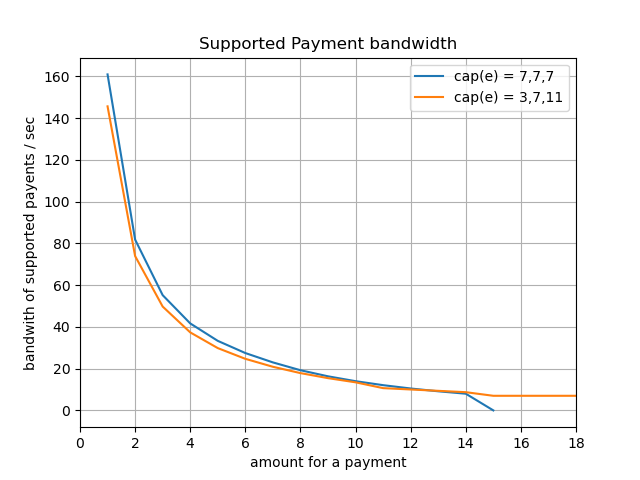
\includegraphics[width=0.41\textwidth]{paymentrate}
\caption{Rate of infeasible payments \( \rho \) depending on the desired payment amount \( a \) in the example network between Alice, Bob, and Carol with channels of sizes 3, 7, and 11}
\label{fig:bandwidth}
\end{figure}

Using the data from Figure \ref{fig:infeasible} we can derive $\mathcal{S}$ for various networks and payment amounts which is depicted in figure \ref{fig:bandwidth}
The figure also demonstrates what users of payment channel networks have experienced before:
Such networks are mainly capable to scale the bandwidth of small amount payments.
There seems a small tradeoff between higher bandwidth but smaller supported maximum sendable amounts for networks with equally sized channels.
We will see later in this document how multiparty channel networks values of \( r(G) \) that are close to $1$.

\section{Relation between the Polytope $L_G$ of Liquidity States and $W_G$ of feasible Wealth Distributions}
Given the topology of the lightning network as a weighted, undirected graph $G(V,E,cap)$.
There is a geometric relation between the corresponding polytopes $L_G$ of liquidity states and $W_G$ of feasible wealth distributions.
For every feasable state $\lambda \in L_G$ we have seen that the $n$ participants $\{v_1,\dots,v_n\}$ have a non negative wealth stored in their channels.
Thus we can project any liquidity state to a feasible wealth distribution via the projection:

\begin{equation}
  \begin{split}
  \label{eq:pi}
  \pi: L_G & \longrightarrow {W_G}\\
  \lambda & \stackrel{\pi}{\longmapsto}\sum_{e=(u,v)\in E}\left(\lambda(e,u)\cdot b_u + \lambda(e,v)\cdot b_v\right)
  \end{split}
\end{equation}

We proof that the image of $\pi$ is indeed a subset of $W_G$. To do this we show that $\pi(\lambda)$ is feasible in $W_G$.

\begin{lemma}
Let $w = \pi(\lambda)$. For a given base we can write $w=\sum_{v\in V}w_v\cdot b_v$. Then $\sum_{v\in V}w_v = C$ 
\end{lemma}
\begin{proof}
  We use the definition of our projection $\pi$ in equation \ref{eq:pi} as well as conservation of liquidity (equation \ref{eq:conservationOfLiquidity}) and the definition of $C$:

\begin{equation}
\begin{split}
  \sum_{v\in V}w_v & = \sum_{v\in V}\sum_{e\in E:v \in e}\lambda(e,v) \\
  & = \sum_{e\in E}\sum_{v\in e}\lambda(e,v) \\
  & = \sum_{e\in E} c_{e} \\
  & = C
\end{split}
\end{equation}
\end{proof}

%% Because of the methods introduced in section \ref{sec:isomorphism} we can find a preimage of $w\in W_G$ under $\pi$.
%% Thus $\pi$ is surjective. 
%% In topology any surjective map induces an equivalence relation from which a quotiont space can be constructed.

%% \begin{definition}
%% We call two states $\lambda,\mu\in L_G$ equvalent if and only they are projected to the same wealth distribution id est: $\pi(\lambda)=\pi(\mu)$.
%% In this case we write $\lambda\sim_{\pi}\mu$.
%% \end{definition}

%% \begin{lemma}
%% The relation $\sim_{\pi}$ is an equivalance relation. In particular it is reflexive, symmetrical and transitve.
%% \end{lemma}
%% \begin{proof}
%%   We need to show that the three properties for an equivalence relation are fulfilled:
%%   \begin{enumerate}
%%   \item \textbf{Reflexivity:} Because $\pi(\lambda)=\pi(\lambda)$ we have $\lambda\sim_{\pi}\lambda$ for any $\lambda \in L_G$.
%%   \item \textbf{Symmetry:} Let $\lambda,\mu\in L_G$ with $\lambda\sim_{\pi}\mu$ which means that $\pi(\lambda)=\pi(\mu)$. Because equality is symmetical it follwos that $\pi(\mu)=\pi(\lambda)$ which means that $\mu\sim_{\pi}\lambda$
%%   \item \textbf{Transitivity:} Let $\lambda,\mu,\nu\in L_G$ with $\lambda\sim_{\pi}\mu$ and $\mu\sim_{\pi}\nu$. We have $\pi(\lambda) = \pi(\mu) = \pi(\nu)$ from which it follows that $\lambda\sim_{\pi}\nu$.
%%   \end{enumerate}
  
%% \end{proof}

Due to the methods introduced in Section \ref{sec:isomorphism}, we can find a preimage of \( w \in W_G \) under \( \pi \).  
Thus, \( \pi \) is surjective.  
In topology, any surjective map induces an equivalence relation, from which a quotient space can be constructed.  

\begin{definition}
We call two states \( \lambda, \mu \in L_G \) equivalent if and only if they are projected to the same wealth distribution, i.e., \( \pi(\lambda) = \pi(\mu) \).  
In this case, we write \( \lambda \sim_{\pi} \mu \).
\end{definition}

\begin{lemma}
The relation \( \sim_{\pi} \) is an equivalence relation. In particular, it is reflexive, symmetrical, and transitive.
\end{lemma}

\begin{proof}
We need to show that the three properties of an equivalence relation are fulfilled:
\begin{enumerate}
    \item \textbf{Reflexivity:} Since \( \pi(\lambda) = \pi(\lambda) \), we have \( \lambda \sim_{\pi} \lambda \) for any \( \lambda \in L_G \).
    \item \textbf{Symmetry:} Let \( \lambda, \mu \in L_G \) with \( \lambda \sim_{\pi} \mu \), which means \( \pi(\lambda) = \pi(\mu) \). Since equality is symmetrical, it follows that \( \pi(\mu) = \pi(\lambda) \), which means \( \mu \sim_{\pi} \lambda \).
    \item \textbf{Transitivity:} Let \( \lambda, \mu, \nu \in L_G \) with \( \lambda \sim_{\pi} \mu \) and \( \mu \sim_{\pi} \nu \). We have \( \pi(\lambda) = \pi(\mu) = \pi(\nu) \), from which it follows that \( \lambda \sim_{\pi} \nu \).
\end{enumerate}
\end{proof}

%% \begin{definition}
%% We call $[\lambda] = \{\mu \in L_G | \lambda\sim_{\pi} \mu\}$ the equivalence class of $\lambda$.
%% The quotient space $L_G/\sim_{\pi}$ is the space of equivalence classes.
%% \end{definition}

%% In particular the equivalence class $[\lambda]=\pi^{-1}(\{w\})$ is the preimage of $w\in W_G$ under the projection $\pi$. 
%% It follows that
%% \begin{equation}
%%   L_G/\sim_{\pi}\cong W_G
%% \end{equation}
%% for which we have explicitly provided the isomorphism.
%% In one direction it is just the projection of the channel states to the wealth distribution as defined in $\pi$ and in the other direction it is constructing a feasible state for a feasible wealth distribution as described in section \ref{sec:isomorphism}.

\begin{definition}
We call \( [\lambda] = \{\mu \in L_G \mid \lambda \sim_{\pi} \mu\} \) the equivalence class of \( \lambda \).  
The quotient space \( L_G / \sim_{\pi} \) is the space of equivalence classes.
\end{definition}

In particular, the equivalence class \( [\lambda] = \pi^{-1}(\{w\}) \) is the preimage of \( w \in W_G \) under the projection \( \pi \).  
It follows that
\begin{equation}
  L_G / \sim_{\pi} \cong W_G
\end{equation}
for which we have explicitly provided the isomorphism.  
In one direction, it is the projection of the channel states to the wealth distribution as defined by \( \pi \), and in the other direction, it is the construction of a feasible state for a feasible wealth distribution as described in Section \ref{sec:isomorphism}.

\subsection{Rebalancing Payment Channels and Circulations}
%% We wish to study the number of elements in the equivalance class $|[\lambda]|$.
%% Remember for $\lambda,\mu\in[\lambda]$ we have: $\pi(\lambda)=\pi(\mu)$.
%% Thus $\lambda$ and $\mu$ are projected to the same wealth distribution. 
%% If routing fees are being ignored circular self payments which are also known as channel rebalancings are the only payments that do not change the wealth distribution.
%% They do however change the liquidity state of the network.

%% We will now proof that the size of the equivalence class $|[\lambda]|$ is equal to the number of stricht circulations that exist on $\mathcal{L}(G,\lambda)$.
%% Also if $\pi(\lambda)=w$ then $|\pi^{-1}(\{w\})|$ is equal to the number of circulations.\footnote{We are not the first to note that circular self payments do not change the wealth distributions \cite{piatkivskyi2018rebalancing} of the participants of a payment channel network.}
%% Counting the number of circulations is possible with Ehrhart's theory\cite{ehrhart1962polyhedra} or by applying Barvinok's algorithm\cite{barvinok1994polynomial}.
%% In particular free open source software\footnote{\url{https://www.math.ucdavis.edu/~latte/}} exists\cite{de2004effective} that is able to achieve this.

%% In order to follow this observations we review a few elements from the theory of network flows.
%% \begin{definition}
%% A flow network is a directed graph \( G = (V, E) \) with capacity function \( c: E \rightarrow \mathbb{Z}^+ \) and flow function \( f: E \rightarrow \mathbb{Z} \) such that \( 0 \leq f(e) \leq c(e) \) for all \( e \in E \).
%% \end{definition}
%% Some flows are of particular interest: 
%% \begin{definition}
%%   A flow \( f \) where the flow conservation constraints are satisfied at every vertex \( x \in V \), i.e.,
%%   \begin{equation}
%%     \sum_{(u,x) \in E} f(u,x) = \sum_{(x,v) \in E} f(x,v)
%%   \end{equation}
%% is called a circulation.
%% \end{definition}

We aim to study the number of elements in the equivalence class \( |[\lambda]| \).  
Recall that for \( \lambda, \mu \in [\lambda] \), we have \( \pi(\lambda) = \pi(\mu) \).  
Thus, \( \lambda \) and \( \mu \) project to the same wealth distribution.  
When routing fees are ignored, circular self-payments, also known as channel rebalancings, are the only payments that do not change the wealth distribution.  
However, they do alter the liquidity state of the network.  

We will now prove that the size of the equivalence class \( |[\lambda]| \) is equal to the number of strict circulations that exist on \( \mathcal{L}(G, \lambda) \).  
Also, if \( \pi(\lambda) = w \), then \( |\pi^{-1}(\{w\})| \) is equal to the number of circulations.\footnote{We are not the first to note that circular self-payments do not change the wealth distributions of the participants in a payment channel network \cite{piatkivskyi2018rebalancing}.}  
Counting the number of circulations is possible with Ehrhart's theory \cite{ehrhart1962polyhedra} or by applying Barvinok's algorithm \cite{barvinok1994polynomial}.  
In particular, free open source software\footnote{\url{https://www.math.ucdavis.edu/~latte/}} exists \cite{de2004effective} that can achieve this.  

To follow these observations, we review a few elements from the theory of network flows.  

\begin{definition}
A flow network is a directed graph \( G = (V, E) \) with a capacity function \( c: E \rightarrow \mathbb{Z}^+ \) and a flow function \( f: E \rightarrow \mathbb{Z} \) such that \( 0 \leq f(e) \leq c(e) \) for all \( e \in E \).
\end{definition}

Certain flows are of particular interest:  

\begin{definition}
A flow \( f \) is called a circulation if at every vertex \( x \in V \) we have:
\begin{equation}
\sum_{(u,x) \in E} f(u,x) = \sum_{(x,v) \in E} f(x,v)
\end{equation}
\end{definition}

%% Because of the particular way how we created the liquidity graph $\mathcal{L}(G,\lambda)$ we need to get a stricter definition for circulations.

%% \begin{definition}
%%   On bidirectional flow Networks where for any $(u,v)\in E$ there is also $(v,u)\in E$ we call a circulation $f$ strict if for all edges $(u,v)\in E$ we have either $f(u,v)=0$ or $f(v,u)=0$ or both $f(u,v)=0=f(v,u)$.
%% \end{definition}

%% We now show that there is a $1$ to $1$ correspondence between strict circulations on $\mathcal{L}(G,\lambda)$ and the elements of $[\lambda]$.
%% First, let $f$ be a circulation on $\mathcal{L}(G,\lambda)$.
%% We show that $\lambda'$ that is defined pointwise for every $e=(u,v)$ through
%%   \begin{equation}
%%   \lambda'(e,u) = \lambda(e,u) + f(v,u) - f(u,v)
%%   \end{equation}
%%   and
%%   \begin{equation}
%%   \lambda'(e,v) = \lambda(e,v) + f(u,v) - f(v,u)
%%   \end{equation}
%%   is indeed a member of $[\lambda]$.
%%   For this we proof the following lemma.

%% \begin{lemma}
%%   Let $G(V,E,cap)$ be a payment channel network in an arbitrary feasible state $\lambda\in L_G$.
%%   Then $\lambda'\in L_G$ and in particular $\pi(\lambda)=\pi(\lambda')$.
%% %  If the flow function $f$ on the liquidity network $\mathcal{L}(G,\lambda)$ is a circulation then $\pi(\lambda') = \pi(\lambda)$ for 
%% \end{lemma}
%% \begin{proof}
%%   We use the fact tha $\lambda \in L_G$ and conservation of liquidity to show that conservation of liquidity also holds for $\lambda'$: 
Due to the particular construction of the liquidity graph \(\mathcal{L}(G,\lambda)\), we require a more precise definition of circulations.

\begin{definition}
  In bidirectional flow networks, where for any \((u,v) \in E\) there is also \((v,u) \in E\), a circulation \(f\) is called strict if for all edges \((u,v) \in E\), we have either \(f(u,v) = 0\) or \(f(v,u) = 0\), or both \(f(u,v) = 0 = f(v,u)\).
\end{definition}

We now demonstrate that there is a one-to-one correspondence between strict circulations on \(\mathcal{L}(G,\lambda)\) and the elements of \([\lambda]\).  
First, let \(f\) be a circulation on \(\mathcal{L}(G,\lambda)\).  
We show that \(\lambda'\), defined pointwise for every \(e = (u,v)\) by
\begin{equation}
  \lambda'(e,u) = \lambda(e,u) + f(v,u) - f(u,v)
\end{equation}
and
\begin{equation}
  \lambda'(e,v) = \lambda(e,v) + f(u,v) - f(v,u),
\end{equation}
is indeed a member of \([\lambda]\).  
To establish this, we prove the following lemma.

\begin{lemma}
  Let \(G(V,E,cap)\) be a payment channel network in an arbitrary feasible state \(\lambda \in L_G\).  
  Then \(\lambda' \in L_G\) and, in particular, \(\pi(\lambda) = \pi(\lambda')\).
\end{lemma}
\begin{proof}
  We use the fact that \(\lambda \in L_G\) and conservation of liquidity to show that conservation of liquidity also holds for \(\lambda'\):
%%%%% HERE CHAT GPT TRIED TO PROOF THE THEOREM. thile the computation is correct it doesn't proof the lemma. It can be used at a later spot though
  %% \begin{equation}
  %%   \sum_{e \in E: v \in e} \lambda'(e,v) = \sum_{e \in E: v \in e} \left(\lambda(e,v) + f(u,v) - f(v,u)\right)
  %% \end{equation}
  %% By definition of a strict circulation, this simplifies to:
  %% \begin{equation}
  %%   \sum_{e \in E: v \in e} \lambda(e,v) + \sum_{e \in E: v \in e} f(u,v) - \sum_{e \in E: v \in e} f(v,u)
  %% \end{equation}
  %% Given that \(f\) is a circulation, the net flow is zero, and we get:
  %% \begin{equation}
  %%   \sum_{e \in E: v \in e} \lambda(e,v) = \sum_{e \in E: v \in e} \lambda'(e,v)
  %% \end{equation}
  %% Thus, conservation of liquidity holds for \(\lambda'\) and therefore \(\lambda' \in L_G\).  
  %% Since \(\pi(\lambda') = \pi(\lambda)\), \(\lambda'\) belongs to the equivalence class \([\lambda]\).
%\end{proof}

\begin{equation*}
    \begin{split}
      \lambda'(e,u) + \lambda'(e,v) & = \lambda(e,u) + f(v,u) - f(u,v) \\
       & + \lambda(e,v) + f(u,v) - f(v,u)\\
      & = \lambda(e,u) + \lambda(e,v) \\
      & + \underbrace{f(u,v) - \underbrace{f(v,u) + f(v,u)}_{=0} - f(u,v)}_{=0}\\
      & = \lambda(e,u) + \lambda(e,v) \\
      & = cap(e)
    \end{split}
  \end{equation*}
  Furhter more we have: 
  \begin{equation}
    \lambda'(e,u) = \underbrace{\lambda(e,u) - \underbrace{f(u,v)}_{\leq \lambda(e,u)}}_{\geq 0} +\underbrace{f(v,u)}_{\geq 0} \geq 0
  \end{equation}
and
  \begin{equation}
    \lambda'(e,u) = \underbrace{\lambda(e,u) + \underbrace{f(v,u)}_{\leq cap(e) - \lambda(e,u)}}_{\leq cap(e)} -\underbrace{f(u,v)}_{\geq 0} \leq cap(e)
  \end{equation}
  This shows that $0\leq \lambda'(e,u) \leq cap(e)$ indicating $\lambda'\in L_G$
  
%%   To show that $\pi(\lambda)=\pi(\lambda')$ we recall the definition of $\lambda'$:
%%     $$\lambda' = \lambda + \underbrace{\sum_{(u,v)\in E'}\left(f(u,v)\cdot b_{(u,v),u} - f(u,v)\cdot b_{(u,v),v}\right)}_{\mu}$$
%%   Since $\pi$ is linear we have $\pi(\lambda') = \pi(\lambda) + \pi(\mu)$.
%%   Thus to show equality of $\pi(\lambda)=\pi(\lambda')$ it is sufficient to test $0\stackrel{!}{=}\pi(\mu)$

%%   \begin{equation}
%%     \begin{split}
%%     \pi(\mu) & =\sum_{(u,v)\in E}\left(f(u,v)\cdot b_u - f(u,v)\cdot b_v\right)
%%     \end{split}
%%   \end{equation}
%%   in particular the $x$-th component of $\pi(\mu)$ can be written as:
%%   $$(\pi(\mu))_x = \sum_{(x,v)\in E}f(x,v) - \sum_{(u,x)\in E}f(u,x)$$
%%   Because of conservation of flow and $f$ being a circulation this equation is $0$ and thus $(\pi(\mu))_x=0$.
%%   Therefor $\pi(\mu)=0$ and $\pi(\lambda)=\pi(\lambda')$
%% \end{proof}
To show that \(\pi(\lambda) = \pi(\lambda')\), we recall the definition of \(\lambda'\):
\[ \lambda' = \lambda + \underbrace{\sum_{(u,v) \in E} \left(f(u,v) \cdot b_{(u,v),u} - f(u,v) \cdot b_{(u,v),v}\right)}_{\mu} \]
Since \(\pi\) is linear, we have \(\pi(\lambda') = \pi(\lambda) + \pi(\mu)\). Thus, to show \(\pi(\lambda) = \pi(\lambda')\), it is sufficient to prove that \(\pi(\mu) = 0\).

\begin{equation}
    \begin{split}
    \pi(\mu) &= \sum_{(u,v) \in E} \left(f(u,v) \cdot b_u - f(u,v) \cdot b_v\right)
    \end{split}
\end{equation}

In particular, for an arbitrary $x\in V$ the \(x\)-th component of \(\pi(\mu)\) can be written as:
\[ (\pi(\mu))_x = \sum_{(x,v) \in E} f(x,v) - \sum_{(u,x) \in E} f(u,x) \]

Because of the conservation of flow and \(f\) being a circulation, this equation equals zero, so \((\pi(\mu))_x = 0\).

Therefore, \(\pi(\mu) = 0\) and \(\pi(\lambda) = \pi(\lambda')\).
\end{proof}
  
%% After we have seen that a circulation $f$ on $\mathcal{L}(G,\lambda)$ gives us a new liquidity state $\lambda'$ we want to show that the provided mapping is injective.
%% \begin{lemma}
%%   Let $f\neq g$ be strict circulations on $\mathcal{L}(G,\lambda)$ then the associated liquidity states $\lambda_f\neq \lambda_g$.
%% \end{lemma}
%% \begin{proof}
%%   We proof this by contradiction:
%%   Assume $\lambda_f = \lambda_g$.
%%   This means $\forall e=(u,v)\in E$ we have:
%%   \begin{equation*}
%%     \begin{split}
%%   \lambda(e,u) + f(v,u)-f(u,v) & = \lambda(e,u) + g(v,u)-g(u,v)\\
%%   \Leftrightarrow f(v,u) - f(u,v) & = g(v,u) - g(u,v)
%%   \end{split}
%%   \end{equation*}
%%   Because $f$ and $g$ were strict circulations at least one term on each side of the equations equals to zero.
%%   Thus we look at all cases.
%%   The $3^{rd}$ and $4^{th}$ case will make use of the fact that $f,g\geq 0$.\\
%%   \textbf{1. case}:
%%   $$f(v,u) = g(v,u) = 0 \Rightarrow -f(u,v) = -g(u,v)$$
%%   \textbf{2. case}:
%%   $$f(u,v) = g(u,v) = 0 \Rightarrow f(v,u) = g(v,u)$$
%%   \textbf{3. case}:
%%   $$f(v,u) = g(u,v) = 0 \Rightarrow -f(u,v) = g(v,u) = 0$$
%%   \textbf{4. case}:
%%   $$f(u,v) = g(v,u) = 0 \Rightarrow f(v,u) = -g(u,v) = 0$$

%%   This shows that $f=g$ which is a contradiction to $f\neq g$.
%%   Thus $\lambda_f \neq \lambda_g$.
%% \end{proof}

%% Finally we proof that our correspondance is between strict circulations and equivalent liquidity states is surjective.
%% \begin{lemma}
%%   For any $\lambda'\in[\lambda]$ there exists a strict circulation $f$ on $\mathcal{L}(G,\lambda)$ such that $\lambda'(u,v)=\lambda(u,v) + f(v,u) - f(u,v)$
%% \end{lemma}
After establishing that a circulation \(f\) on \(\mathcal{L}(G,\lambda)\) results in a new liquidity state \(\lambda'\), we aim to show that the provided mapping is injective.

\begin{lemma}
  Let \(f \neq g\) be strict circulations on \(\mathcal{L}(G,\lambda)\). Then the associated liquidity states \(\lambda_f \neq \lambda_g\).
\end{lemma}

\begin{proof}
  We prove this by contradiction.
  Assume \(\lambda_f = \lambda_g\).
  This means that for all \(e = (u,v) \in E\), we have:
  \begin{equation*}
    \begin{split}
      \lambda(e,u) + f(v,u) - f(u,v) &= \lambda(e,u) + g(v,u) - g(u,v) \\
      \Leftrightarrow f(v,u) - f(u,v) &= g(v,u) - g(u,v)
    \end{split}
  \end{equation*}
  Because \(f\) and \(g\) are strict circulations, at least one term on each side of the equation equals zero. We consider all cases, noting that \(f,g \geq 0\):

  \textbf{1. Case:}
  \[ f(v,u) = g(v,u) = 0 \Rightarrow -f(u,v) = -g(u,v) \]

  \textbf{2. Case:}
  \[ f(u,v) = g(u,v) = 0 \Rightarrow f(v,u) = g(v,u) \]

  \textbf{3. Case:}
  \[ f(v,u) = g(u,v) = 0 \Rightarrow -f(u,v) = g(v,u) = 0 \]

  \textbf{4. Case:}
  \[ f(u,v) = g(v,u) = 0 \Rightarrow f(v,u) = -g(u,v) = 0 \]

  This shows that \(f = g\), which contradicts our assumption that \(f \neq g\). Therefore, \(\lambda_f \neq \lambda_g\).
\end{proof}

Finally, we prove that our correspondence between strict circulations and equivalent liquidity states is surjective.

\begin{lemma}
  For any \(\lambda' \in [\lambda]\), there exists a strict circulation \(f\) on \(\mathcal{L}(G,\lambda)\) such that \(\lambda'(u,v) = \lambda(u,v) + f(v,u) - f(u,v)\).
\end{lemma}
%% \begin{proof}
%%   Now for any $e=(x,y)$ we set:
%% \begin{equation}
%%   f(x,y) =\begin{cases}
%%         \lambda(e,x)-\lambda'(e,x) & \text{if $  \lambda(e,x) \geq\lambda'(e,x)$}\\
%%       0 & \text{otherwise}
%%     \end{cases}
%%   \end{equation}
%% From definition it follows that:
%% $$0\leq f(x,y) \leq c(x,y)$$

%%   The $x$-th component of the welth vector $\pi(\lambda)$ is computed as:
%%   $$\left(\pi(\lambda)\right)_x = \sum_{e\in E: x\in e}\lambda(e,x)$$
%%   Since $\lambda'\in [\lambda]$ we have $\pi(\lambda') = \pi(\lambda)$
%%   if follows for any $x\in V$:
%%   $$0 = \sum_{e\in E: x\in e}\left(\lambda(e,x)-\lambda'(e,x)\right)$$
%% If $\lambda(e,x)-\lambda'(e,x) \geq 0$ then we have:
%% $$f(x,y) = \lambda(e,x)-\lambda'(e,x)$$
%% Otherwise we can use conservation of liquidity to show:
%% \begin{equation*}
%%   \begin{split}
%%   \lambda(e,x)-\lambda'(e,x) & = cap(e) - \lambda(e,y) - \left(cap(e) - \lambda'(e,y)\right)\\
%%   & = cap(e) - \lambda(e,y) - cap(e) + \lambda'(e,y)\\
%%   & = - \lambda(e,y) + \lambda'(e,y)\\
%%   & = -\underbrace{\left(\lambda(e,y) - \lambda'(e,y)\right)}_{f(y,x)}\\
%%   & = -f(y,x)
%%   \end{split}
%%   \end{equation*}
%% Therefor we can replace $\lambda(e,x)-\lambda'(e,x)$ with $f(x,y)-f(y,x)$ and we get.
%% \begin{equation}
%%   \begin{split}
%% 0 & = \sum_{e\in E: x\in e}\left(\lambda(e,x)-\lambda'(e,x)\right)\\
%% & = \sum_{e\in E:x\in e}\left(f(x,y) - f(y,x)\right) \\
%% & = \sum_{e\in E:x\in e}f(x,y) -\sum_{e\in E:x\in e} f(y,x)\\
%% & \Leftrightarrow  \sum_{(y,x)}f(y,x)  =\sum_{(x,y)} f(x,y)\\
%%   \end{split}
%% \end{equation}
%% This proofs that $f$ was a strict circulation on $\mathcal{L}(G,\lambda)$.
%%   \end{proof}

%% We from those lemmas the main theorem follows:
%% \begin{theorem}
%%   The fiber $\pi^{-1}(\{w\})$ of any feasible wealth distribution $w\in W_G $ is an equivalence class $[\lambda]$ of liquidity states.
%%   The number of strict circulations on $\mathcal{L}(G,\lambda)$ is the same as the number $|[\lambda]|$ of distinct liquidity states of the network with the same fixed wealth distributin $w\in W_G$.
%% \end{theorem}
%% Circular rebalancing of liquidity does not change the feasibility of a payment as circulations leave the wealth distribution invariant and feasibility of payments is decided by testing if the change in wealth distribution is sill a feasible wealth distribution.
%% However depending which liquidity state $\lambda\in\pi^{-1}(\{w\})$ the network is in has an impact how quickly payment planning strategies of nodes will be able to find the necessary liquidity of feasible payments. 
\begin{proof}
For any \(e = (x, y)\), we define:
\[
f(x, y) = 
\begin{cases}
    \lambda(e, x) - \lambda'(e, x) & \text{if } \lambda(e, x) \geq \lambda'(e, x) \\
    0 & \text{otherwise}
\end{cases}
\]
From the definition, it follows that:
\[
0 \leq f(x, y) \leq c(x, y)
\]

The \(x\)-th component of the wealth vector \(\pi(\lambda)\) is computed as:
\[
\left(\pi(\lambda)\right)_x = \sum_{e \in E: x \in e} \lambda(e, x)
\]
Since \(\lambda' \in [\lambda]\), we have \(\pi(\lambda') = \pi(\lambda)\). It follows for any \(x \in V\):
\[
0 = \sum_{e \in E: x \in e} \left(\lambda(e, x) - \lambda'(e, x)\right)
\]

If \(\lambda(e, x) - \lambda'(e, x) \geq 0\), then we have:
\[
f(x, y) = \lambda(e, x) - \lambda'(e, x)
\]

Otherwise, we use the conservation of liquidity to show:
\begin{equation*}
    \begin{split}
        \lambda(e, x) - \lambda'(e, x) &= c(e) - \lambda(e, y) - \left(c(e) - \lambda'(e, y)\right) \\
        &= c(e) - \lambda(e, y) - c(e) + \lambda'(e, y) \\
        &= -\lambda(e, y) + \lambda'(e, y) \\
        &= -\underbrace{\left(\lambda(e, y) - \lambda'(e, y)\right)}_{f(y, x)} \\
        &= -f(y, x)
    \end{split}
\end{equation*}

Therefore, we can replace \(\lambda(e, x) - \lambda'(e, x)\) with \(f(x, y) - f(y, x)\), yielding:
\begin{equation}
    \begin{split}
        0 &= \sum_{e \in E: x \in e} \left(\lambda(e, x) - \lambda'(e, x)\right) \\
        &= \sum_{e \in E: x \in e} \left(f(x, y) - f(y, x)\right) \\
        &= \sum_{e \in E: x \in e} f(x, y) - \sum_{e \in E: x \in e} f(y, x) \\
        &\Leftrightarrow \sum_{(y, x)} f(y, x) = \sum_{(x, y)} f(x, y)
    \end{split}
\end{equation}

This proves that \(f\) is a strict circulation on \(\mathcal{L}(G, \lambda)\).
\end{proof}

From these lemmas, the main theorem follows:

\begin{theorem}
  \label{thm:circulations}
    The fiber \(\pi^{-1}(\{w\})\) of any feasible wealth distribution \(w \in W_G\) is an equivalence class \([\lambda]\) of liquidity states. The number of strict circulations on \(\mathcal{L}(G, \lambda)\) is the same as the number \(|[\lambda]|\) of distinct liquidity states of the network with the same fixed wealth distribution \(w \in W_G\).
\end{theorem}

Circular rebalancing of liquidity does not change the feasibility of a payment since circulations leave the wealth distribution invariant, and the feasibility of payments is determined by testing if the change in wealth distribution still results in a feasible wealth distribution. However, depending on which liquidity state \(\lambda \in \pi^{-1}(\{w\})\) the network is in, the speed at which payment planning strategies of nodes can find the necessary liquidity for feasible payments can be impacted.

\begin{figure}[h]
  \centering
  \hspace{1.5em}
\subfigure[]{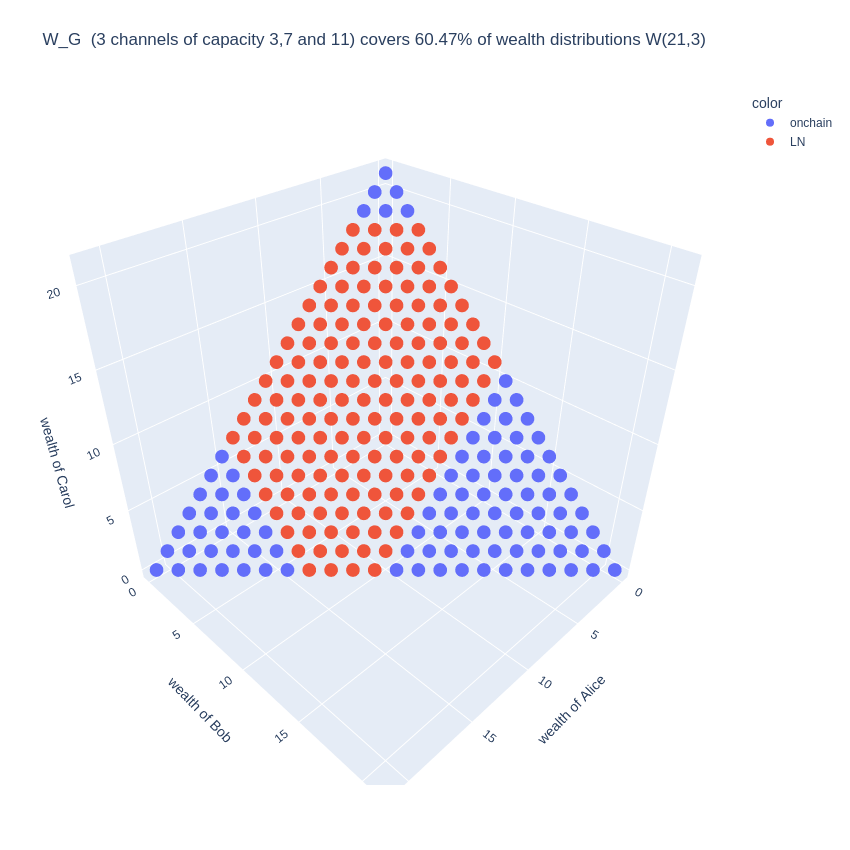
\includegraphics[width=0.152\textwidth]{polytope_of_wealth_distributions_lninequal}}
\hspace{1.5em}
\subfigure[]{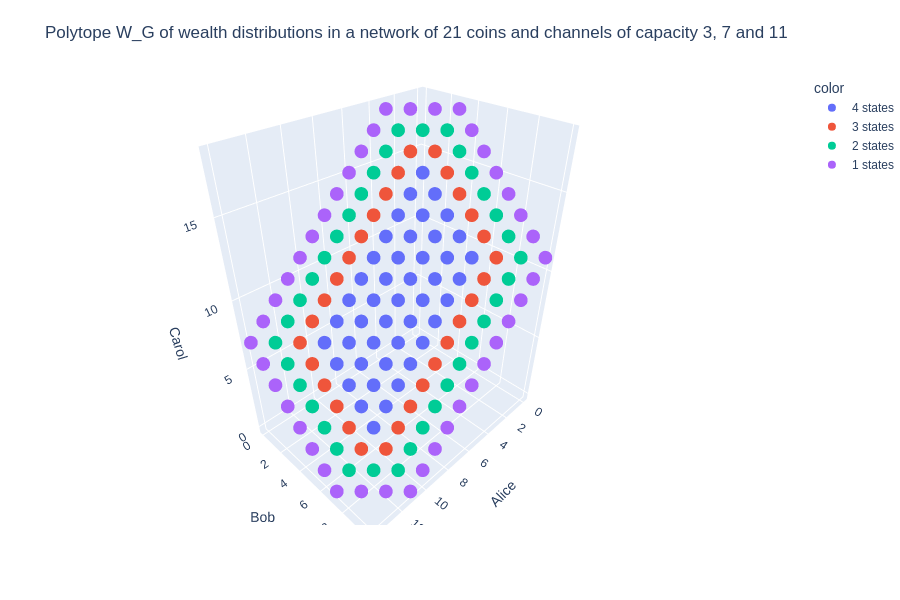
\includegraphics[width=0.23\textwidth]{wdwithstates}}
\subfigure[]{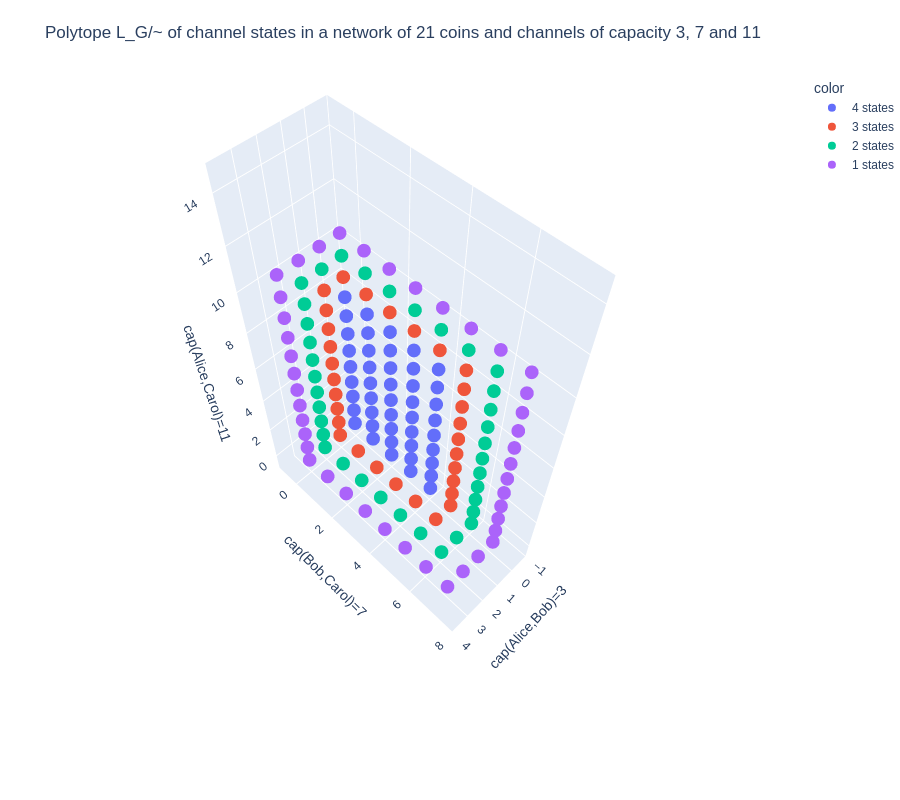
\includegraphics[width=0.23\textwidth]{equivalanceclasses}}
\subfigure[]{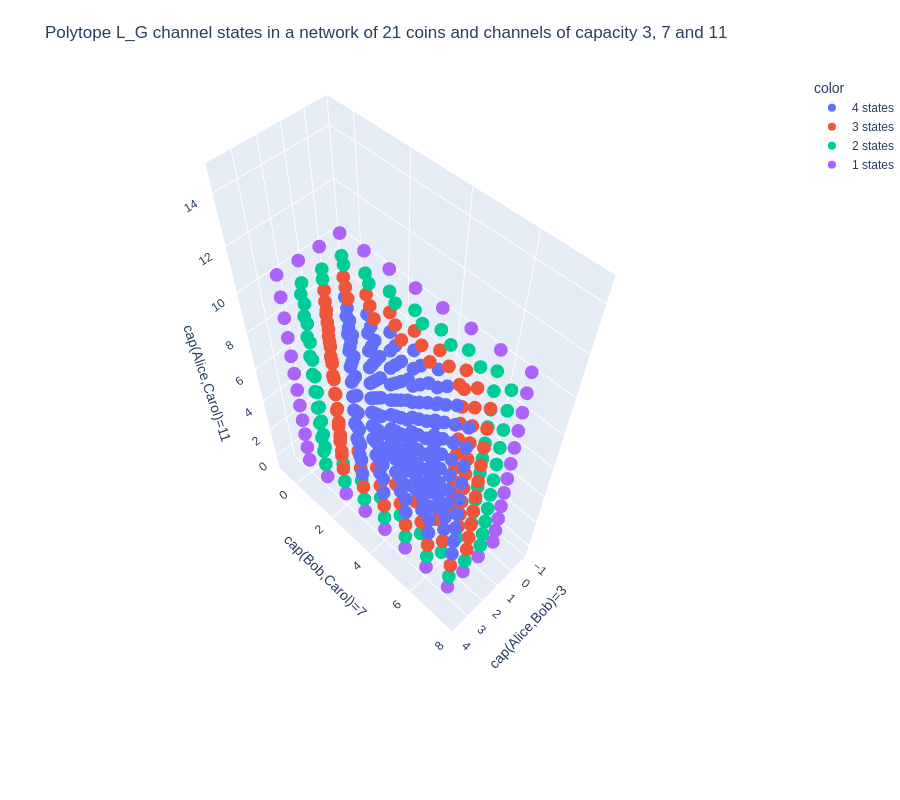
\includegraphics[width=0.23\textwidth]{allstates}}
\caption{(a) shows the feasible region $W_G$ as in figure \ref{fig:feasibleLNWealthPolytopes} (b) depicts the size of the equivalence classe for each feasible wealth distribution. (c) Space $L_G/\sim_\pi$ of equivalance classes as a subset of the surface of $L_G$ (d) full polytope $L_G$ of all liquidity states}
\label{fig:equivalenceclasses}
\end{figure}

Figure \ref{fig:equivalenceclasses} demonstrates in $3$-dimensional geometry how the $L_G$ in combination with $\pi$ can be seen as a bundle over $W_G$ and how $W_G\cong L_G/\sim_\pi$.
In particular in subfigure (c) one can realize that the feasible region $W_G$ corresponds to just $3$ sides of the hypercube:
$$H_G=\{0,1,2,3\}\times\{0,2,3,4,5,6,7\}\times\{0,\dots,11\}$$
Each side corresponds to the subspace in which one dimension (state) equals $0$.
Meaning the liquidity state which is rebalanced so long until one channel is depleted. This obviously works only if cycles are present and not in trees.

\subsection{Special Case of Spanning Trees}
%% Let us assume $G$ had the shape of a tree.
%% In this case
%% $$m = |E| = |V|-1 = n-1$$
%% We recall the dimension of $\sigma(G,\omega)$ was: $m-n+1$.
%% replacing $m$ with $n-1$ we see that the dimension of $\sigma(G,\omega)$ is $m-n+1 = (n-1)+n+1 = n-n + 1-1 = 0$
%% A zero dimensional space is just a single point.
%% If $\omega$ was feasible this point lies in $\W_G$ and the liquidity function is unique.
%% Thus on tree shaped networks there is a one to one correspondance of the set $W_G$ and the set of feasible liquidity functions $L_G$. In particular we can write:
%% $$W_G \cong L_G$$
%% The careful reader may have realized that the polytope of feasible liquidity states $L_G$ in figure \ref{fig:statePolytopeExample} had the same number of points as the feasible reagion $W_G$ in figure \ref{fig:wealthPolytope}.
%% As we have seen this is no surprise but to be expected.

%% This means that for a uniform distribution of feasible wealth distributions in a spanning tree the liquidity in channels would also be uniformly distributed and depletion would not occure.
%% This is remarkable because it has been shown\cite{guidi2019steadystate} that under the assumption of balanced flows there is a stable state in which the liquidity within most channels ist depleted but there is a spanning tree in which the liquidity is uniformly distributed. 

Let us assume \(G\) has the shape of a tree. In this case,
\[ m = |E| = |V| - 1 = n - 1 \]
We recall that the dimension of \(\sigma(G, \omega)\) was: \(m - n + 1\). Replacing \(m\) with \(n - 1\), we see that the dimension of \(\sigma(G, \omega)\) is:
\[ m - n + 1 = (n - 1) - n + 1 = 0 \]
A zero-dimensional space is just a single point. If \(\omega\) is feasible, this point lies in \(W_G\), and the corresponding liquidity function is unique. Thus, in tree-shaped networks, there is a one-to-one correspondence between the set \(W_G\) and the set of feasible liquidity functions \(L_G\). In particular, we can write:
\[ W_G \cong L_G \]
The careful reader may have noticed that the polytope of feasible liquidity states \(L_G\) in Figure \ref{fig:statePolytopeExample} had the same number of points as the feasible region \(W_G\) in Figure \ref{fig:wealthPolytope}. As we have seen, this is not surprising but to be expected.

This means that for a uniform distribution of feasible wealth distributions in a spanning tree, the liquidity in channels would also be uniformly distributed, preventing depletion. This is remarkable because it has been shown \cite{guidi2019steadystate} that under the assumption of balanced flows, there is a stable state in which the liquidity within most channels is depleted, but there is a spanning tree in which the liquidity is uniformly distributed.

\section{Channel Depletion as a Consequence of the Goemetry of Cycles}
\textbf{WARNING! FROM HERE ON THE PAPER NEEDS TO BE REWRITTEN AND FINALIZED}
We have seen that under the assumption that all feasible wealth distributions in $W_G$ are equally likeli that in spanning trees the liquidity states is also uniformly distributed.
In particular the channel states are equally likely and idependent of each other.

In figure \ref{fig:equivalenceclasses} (b) we have seen that the the feasible wealth distributions $w\in W_G$ with $|\lambda|=|\pi^{-1}(\{w\})|$ are located on the boundary of $W_G$.
Assuming every node in the network is part of a cycle then the wealth distributions with $|\lambda|=1$ are because of theorem \ref{thm:circulations} those that do only have the trivial circulation ($f=0$) on the associated liquidity network $\mathcal{L}(G,\lambda)$.
The fact that no other circulations exists means that at least one channel has to be depleted. 
It is a well known fact most of the volume of high dimensional convex bodyes is located close to the boundary.
To see this for an $n$-dimensional hyper we realize that its $n$ dimensional volume is described as:
$$vol = l^n$$
If we want to see how much volume is on the boundary we have to substract the volume of a cube that has a length of $l-2$:
$$vol(boundary) = l^n - (l-2)^n$$
Use concentration of measure to show how depletion has to occur. 

\section{Multiparty channels}
Everyhing we saw generalizes easily to $k$-party channels.
A $k$-party channel is a channel is an element in $V^k$ thus the channels build a subset $E_k\subset V^k$.
The capacity function $cap_k:E_k\longrightarrow \mathbb{N}$ is generalized.
We for $2\leq k\leq n$ we call $G_k(V,E_k,cap_k)$ a $k$-party payment channel network.
If $k==2$ we omit $k$ and just have a regular graph.
Obviously the principle of conservation of liquidity must still hold:
\begin{equation}
cap(e)=\sum_{x\in e}\lambda(e,x) \forall e\in E_k
\end{equation}

Obviously the number of possible $k$ party channels in a network of $n$ participants is defined by:
$${{n}\choose {k}}$$
Thus $|E_k|\leq {{n}\choose {k}}$.

We can easily see that the hypberbox $B$ which describes the variables is $k\cdot m$ dimensional.
If the $m$ linear independent constraints are divided out we get the state polytope $S_k\subset \mathbb{Z}^{(k-1)\cdot m}$.
We again have the cannonical projection $\pi: S\longrightarrow W_{G_k}$ to the polytope of feasible wealth distributions with $k$-party channels.

\begin{definition}
  Let $G_k(V,E_k,cap)$ be a $k$-party channel network.
  We call $G_{k+1}(V,E_{k+1},cap_{k+1})$ an extension if
  $$|E_{k+1}| \leq |E_k|$$
  and
  $$\forall e=\{x_1,\dots,x_k\}\in E_k \hspace{0.25cm}\exists! e'\in E_{k+1} : e\subset e'$$
  and
  $$cap_{k+1}(e') =\sum{e\in\epsilon} cap_k(e)$$
  with $\epsilon=\{e_1,\dots,e_N\}\subset E_k$ be the subset of edges in $E_k$  such that $|e'\backslash e_i|=1$.
  $\epsilon'$ is the set of edges that are being extended to $e'$.
\end{definition}

Graph extensions are useful because we can proof the extensability theorem which indicates that multi party channels allow for more feasible wealth distributions.


\begin{theorem}
  \textbf{Extensability Theorem:} 
  Let $G_{k+1}$ be an extension of $G_{k+1}$ then 
  $$W_{G_k} \subsetneq W_{G_{k+1}}$$
\end{theorem}

\begin{proof}\footnote{I assume one can crate a projection matrix that mapps the constraints from the $k+1$ party channel network down to $k$-party channel networks}
  Let $w\in W_{G_k}$ be a a feasible wealth distribution.
  We need to show that $w\in W_{G_{k+1}}$
  Because $w$ is feasible there exists a feasible state $x\in\pi_k^{-1}(w)$ that satisfisfies the wealth distribution.
  For any edge $e' \in G_{k+1}$
  Beacuse $G_{k+1}$ is an exstension $\epsilon$ has at least one element.
  Now we set:
\begin{equation}
  e'_x = \begin{cases}
      \sum_{e\in\epsilon}e_x & \text{if $\exists e\in\epsilon : x\in e$}\\
      0 & \text{(otherwise)}
    \end{cases}
\end{equation}
$e'$ fulfills conservation of liquidity.
Thus we have constructed a feasible state $x$ in the $(k+1)$-party channel network with $\pi(x)=w$.
This concludes our proof and demonstrates that in the multi party channel extension there are at least as many wealth distributions feasible as before.
\end{proof}
While the communications protocol for multiparty channels are complicated and developer currently avoid implementing such channels several cryptographic secure constructs for multiparty channels exist.

\subsection{Example how multiparty channel network achieves more feasible wealth distributions}
Assume we have $4$ participants bringing $3$ coins each. for $k=2$ we could create the following network:

We have $6$ payment channels of capacity $2$ each and each user is part of $3$ of the $4$ channels.
In particular a user could allocate $1$ coin to each channel.
This topology corresponds to a fully connected graph.
Each user could own at most $6$ coins in this topology.

On the other hand a setup where these $4$ participants select $k=3$ to create $3$-party channels we see that in this particular case at most $4$ such channels are possible.
Each user would be part in $3$ of the $4$ multiparty channels.
Again in this particular topology each user could have broght $1$ coin to each channel where the capacity of the channels is now $3$.
Each user could theoretically own up to $9$ coins in this instantiation of the payment channel network.

Of course fully connected networks - in particluar with a small number of users - are rather artificial. but the fact that in this particular case we need only $4$ instead of $6$ on chain transactions and users can not only have more coins but overall more wealth distributions would be possible.

\section{Emperical Results from Simulations and Experiments}
There are currently a few outdated ipython notebooks on the github repository of this paper.
In those we used a trick to more quickly decide if a wealth distribution is feasible.
Unfortunately this resulted in getting false positives.
We will update this section as soon as the notebooks are fixed

\section{Conclusion}
Generally speaking we seek a preferable\footnote{for some suitable definition of preferable} tradeoff between the expenses to maintain channels and the limits and burden they produce to the feasible wealth distributions for the users of payment channel networks.

We have seen that the two party channel design seems too constraint to allow for capital to be deployed efficiently as too many wealth distributions become infeasible.
In particular it seems unlikely that the rate of infeasible payments can be reduced to a level that the payment channel network can relay on liquidity management through on chain transactions to fulfill all conceivable payment requests.


Because of the concentration of measure we can see that channel depletion is to be expected - which leads to a higher rate of payment attempts - even when delivering feasible payments.
The communities wish to avoid credit in payment channel networks is another reason for an increased rate of infeasible payments. 

While the narrative around the likelihood has shifted from being a peer to peer payment system for end users towards being a peer to peer settlement layer between service providers our results indicate that even a fairly small and professionally run payment channel network probably lacks a sufficient service level in terms of reliability and rate of payments being feasible and might depend on too many on chain transactions to to satisfies the user's requests.

Our results indicte that the idea that a two party Lightning Network can be used as a payment / settlement network between federations seems less promessing than understanding federations as multi party channels.
Instead of connecting federations via two party channels it might seems more promesing to create an open standard for a cross federation / multiparty routing protocol.
Of course this could also come in the form of an extension to the lighting network that allows the creation of multi party payment channels and routing though them. 

In particular we have seen that the average access to capital of users grows linear in the number of peers per channel ($k\cdot\frac{C}{n}$).
Also the Polytope $W_k$ of feasible wealth distributions of a $k$-party channel network is a subset of the polytope $W_{k+1}$ of wealth distributions for any extension of the $k$-party channel network to an $(k+1)$-party channel network.
This is a strong indicator that multi party channels are useful.\footnote{In particular for $k=n$ we have only one large multiparty in which all wealth distributions that are feasible on chain will also be feasible in the payment channel. This is similar to systems like Ark.}

%==========================================================================



\section{Acknowledgements}
This work was funded by Open Sats Inc. and various Patreons. I would like to thank the reviewers of earlier versions. In particular Stefan Richter, Christian Decker, Christian Kuemmerle, Anastasios Sidiropoulos (who pointed out an error in my initial description of the wealth distributions), Elias Roher and bitromortac. Thanks to Rene Treffer for sharing an example with me that indicated how dropping the assumption that liquidity in channels is distributed independently can be used to show how bimodal liquidity distributions emerge.
Furthermore since I am not a native english speaker I passed the manuscript through chatGPT for copy editing and revised its output. My origninal manuscript is as comments in the latex files.

\bibliography{references}
\bibliographystyle{plain}


\appendix

  \section{Low Dimensional Example}
\label{sec:paymentsExample}
We have already seen that for different topologies the feasible region and thus $r(G)$.
For our example we set:
\begin{equation*}
  \begin{split}
    V   & =\{x,y,z\} \\
    E=\{e=(x,y),f & =(y,z), g=(x,z)\}\\
    c_e=3, c_f & =7, c_g=11
  \end{split}
\end{equation*}

We want to see if the wealth vector $w=(5,6,10)$ is feasible in this network.
thus we construct our system of linear equations as.

We have $m$ constraints related to conservation of liquidity.
\begin{align*}
  e_x + e_y  & = c_e \\
  f_y + f_z & = c_f \\
  g_x + g_z & = c_g \\
\end{align*}
and $n$ constraints related to the wealth vector.
\begin{align*}
  e_x +  g_x & = w_x \\
  e_y +  f_y & = w_y \\
  f_z +  g_z & = w_z
\end{align*}
Together this results in the following system of linear equations.
\[
  \left[
    \begin{array}{cccccc}
      1 & 1 & 0 & 0 & 0 & 0 \\
      0 & 0 & 1 & 1 & 0 & 0 \\
      0 & 0 & 0 & 0 & 1 & 1 \\
      1 & 0 & 0 & 0 & 1 & 0 \\
      0 & 1 & 1 & 0 & 0 & 0 \\
      0 & 0 & 0 & 1 & 0 & 1 
    \end{array}
    \right]
\begin{bmatrix}
  e_{x}  \\
  e_{y}  \\
  f_{y}  \\
  f_{z}  \\
  g_{x}  \\
  g_{z}  \\
\end{bmatrix} 
  = \begin{bmatrix}
  c_e\\
  c_f\\
  c_g\\
  w_x\\
  w_y\\
  w_z
\end{bmatrix}
\]
Again we ca replace the variables $e_y, f_z$ and $g_z$ with $e_x, f_y$ and $g_x$ respectively. 
\[
  \left[
    \begin{array}{ccc}
      1 & 0 & 1 \\
      - 1& 1 & 0 \\
      0 & -1 & -1 
    \end{array}
    \right]
\begin{bmatrix}
  e_{x}  \\
  f_{y}  \\
  g_{x}  \\
\end{bmatrix} 
  = \begin{bmatrix}
  w_x\\
  w_y\\
  w_z
  \end{bmatrix}
  - \begin{bmatrix}
  0\\
  c_e\\
  c_f + c_g
  \end{bmatrix}
\]

The solution space is $1$ dimensional and can be parmeterized via:

$$\sigma = \{\begin{pmatrix}0\\w_y-c_e\\w_x\end{pmatrix} + t\cdot\begin{pmatrix}1\\1\\-1\end{pmatrix}\in\mathbb{Z}^3| t\in\mathbb{Z}\}$$

Plugging in the wealth vector $w=(5,6,10)^t$ and the capacities we get:

$$\sigma = \{\begin{pmatrix}0\\3\\5\end{pmatrix} + t\cdot\begin{pmatrix}1\\1\\-1\end{pmatrix}\in\mathbb{Z}^3| t\in\mathbb{Z}\}$$


\begin{figure}[h]
  \label{fig:preimage}
\centering
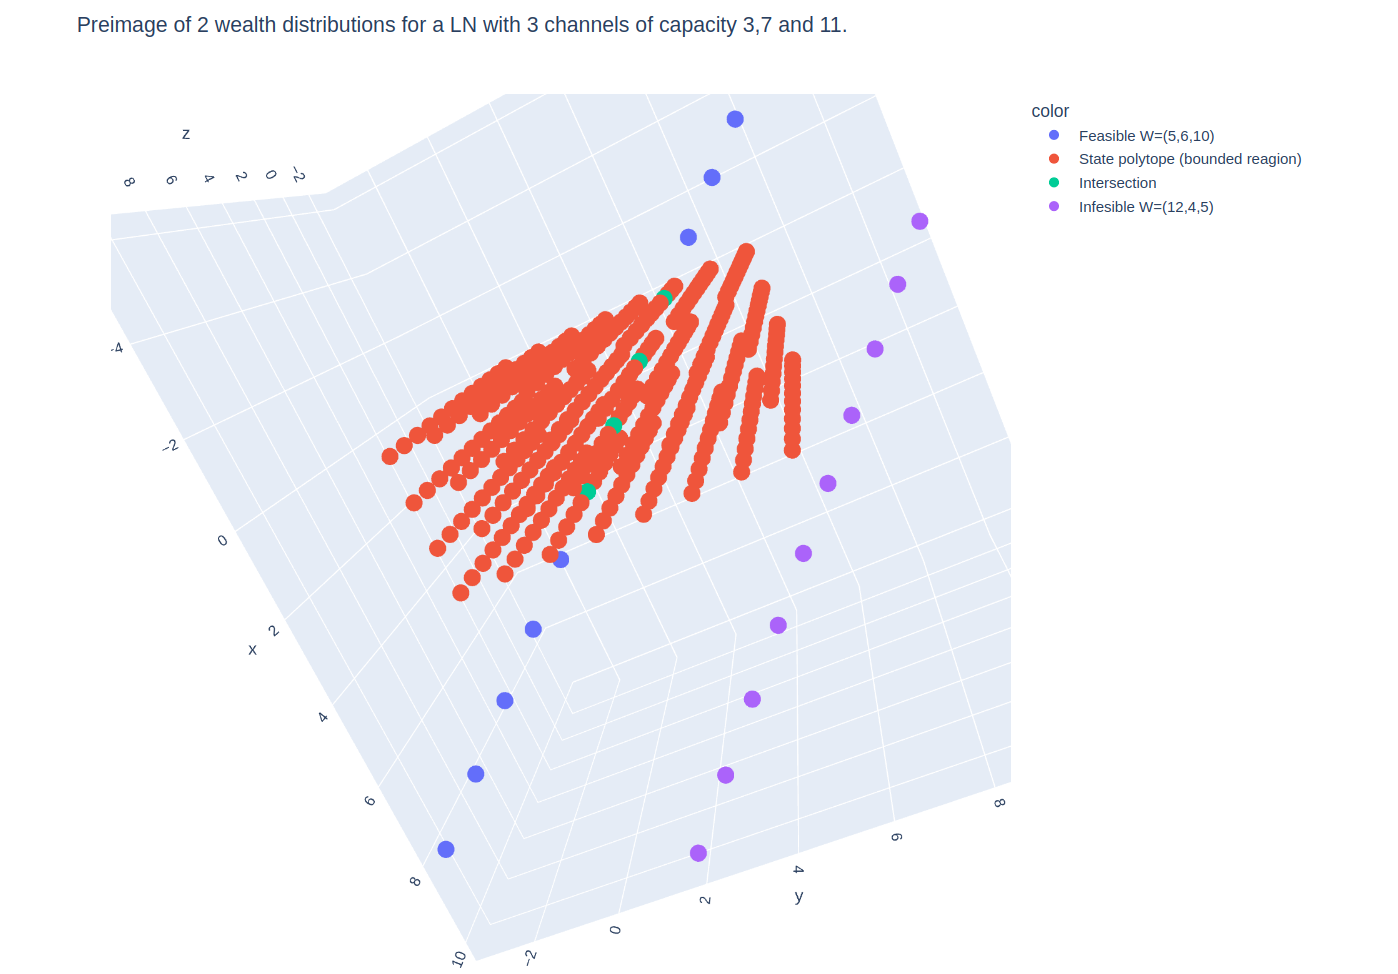
\includegraphics[width=0.5\textwidth]{preimage}
\caption{We see the preimage of $\pi|_{\mathbb{Z}^m}$ for $2$ wealth distributions. One does have an empty intersection with the bounding box of the state polytope and is thus infeasible on the example network.}
\end{figure}

Finally we racall that our state space $S=\{0,\dots,3\}\times\{0,\dots,7\}\times\{0,\dots,11\}$.
We define $F = \sigma\cap S$ to be the set of feasible solutions.
We see that the parameter $t$ cannot be negative. Thus we get the following table of feasible solutions.

%via: https://www.tablesgenerator.com/
% Please add the following required packages to your document preamble:
% \usepackage[table,xcdraw]{xcolor}
% Beamer presentation requires \usepackage{colortbl} instead of \usepackage[table,xcdraw]{xcolor}
\begin{table}[]
\begin{tabular}{|l|c|c|c|c|}
\hline
$t$                                                & $0\leq e_x\leq 3$   & $0\leq f_y\leq 7$   & $0\leq g_x\leq 11$   & \textbf{feasable}        \\ \hline
\rowcolor[HTML]{34FF34} 
\cellcolor[HTML]{FE0000}-1                       & \cellcolor[HTML]{FE0000}-1  & 2                        & 6                        & \cellcolor[HTML]{FE0000}N \\ \hline
\rowcolor[HTML]{34FF34} 
{\color[HTML]{000000} 0}                         & {\color[HTML]{000000} 0}    & {\color[HTML]{000000} 3} & {\color[HTML]{000000} 5} & {\color[HTML]{000000} Y}  \\ \hline
\rowcolor[HTML]{34FF34} 
1                                                & 1                           & 4                        & 4                        & Y                         \\ \hline
\rowcolor[HTML]{34FF34} 
2                                                & 2                           & 5                        & 3                        & Y                         \\ \hline
\rowcolor[HTML]{34FF34} 
3                                                & 3                           & 6                        & 2                        & Y                         \\ \hline
\rowcolor[HTML]{34FF34} 
\cellcolor[HTML]{FE0000}{\color[HTML]{000000} 4} &  \cellcolor[HTML]{FE0000}4  & 7                        & 1                        & \cellcolor[HTML]{FE0000}N \\ \hline
\end{tabular}
\end{table}


If $y$ wants to make a payment of $2$ coins to $z$ we take the wealth vector $w=(5,6,10)^t$ and compute:

\[w'=\begin{pmatrix}5\\6\\10\end{pmatrix}-2\cdot b_y + 2\cdot b_z = \begin{pmatrix}5\\4\\12\end{pmatrix}\]

  We get:
\[\sigma' = \{\begin{pmatrix}0\\1\\5\end{pmatrix}\ + t\cdot \begin{pmatrix}1\\1\\-1\end{pmatrix}\}\]

  For $t=0$ we have $(0,1,5)^t\in S$.
  Thus the wealth distribution $w'\in W$ and the payment was feasible.

  Assuming we have the wealth distribution $w'$ and user $z$ wants to pay $10$ coins to $x$ then we had the wealth distribution $\omega=(15,4,2)$.
  As we have alredy seen in figure \ref{fig:preimage} that the solution space of $\omega$ does have an empty intersection with $S$.
  Thus the payment of $10$ coins is infeasible. 


\section{Open ends}
  \subsection{Conjecture}
  Let $\sigma_w\subset \mathbb{Z}^n$ be the solution space for a wealth distribution $w$.
  Then:
  \begin{equation}
    \frac{|\left(\bigcup_{w\in W}\sigma_w\right)\cap S|}{|S|}
  \end{equation}
  is the liklihood that a payment is infeasible.


  
\subsection{TODO: Compare method to reality and optimally realiable payment flows}
We use a data set of some network probes
However we can estimate the likelihood for a payment to be feasible through statistical sampeling

\subsection{Learn from successfull payments}
if a payment was successfull we can find a subset of feasible states from where we could have started

\subsection{TODO: Compare with min cut distribution}
of course one could also compute the min cut distribution for various uniformly distributed wealth vectors (this is certainly more sound than initilizing channels randomly)

\subsection{understand the subset of equivalence classes}
For a general Network we have:
\begin{equation}
  W_G \cong \bigcup_{i=1}^m\left(H_G\cap\{(\lambda_1,\dots,\lambda_m)\in L_G|\lambda_i = 0\}\right)
  \end{equation}

\subsection{Questions}
\begin{enumerate}
\item Assuming all coins must be put into payment channels with a static topology. How should the capacities of the payment channels for a given wealth distribution being chosen? Is the goal that the space of possible wealth distributions is maximized favourable? 
\item Assume only a limited amount of payment channels can be created (due to the fact that payment channels are achored as multisig transactions in the blockchain which has limited space). What is a desireable topology of channels at blockheight $h$ for a fixed rate of channels per block?
\item Given that a subset of the existing coins may be put in payment channels. How many coins should be used to create channels?
\end{enumerate}

\end {document}

